%
% Modified by Sameer Vijay
% Last Change: Wed Jul 27 2005 13:00 CEST
%
%%%%%%%%%%%%%%%%%%%%%%%%%%%%%%%%%%%%%%%%%%%%%%%%%%%%%%%%%%%%%%%%%%%%%%%%
%
% Sample Notre Dame Thesis/Dissertation
% Using Donald Peterson's ndthesis classfile
%
% Written by Jeff Squyres and Don Peterson
%
% Provided by the Information Technology Committee of
%   the Graduate Student Union
%   http://www.gsu.nd.edu/
%
% Nothing in this document is serious except the format.  :-)
%
% If you have any suggestions, comments, questions, please send e-mail
% to: ndthesis@gsu.nd.edu
%
%%%%%%%%%%%%%%%%%%%%%%%%%%%%%%%%%%%%%%%%%%%%%%%%%%%%%%%%%%%%%%%%%%%%%%%%

%
% Chapter 4
%

\chapter{DATA ANALYSIS}
\label{chap:dataAnalysis}
\begin{comment}
We care about two things:
1. The absolute cross-section of the ground state transition
2. Setting a limit on excited 0+ state cross-sections
\end{comment}
The aim of the analysis of the \reaction data sets is to extract the absolute cross section of the reactions populating the ground states of \SeProducts and also to set as strict a limit on excited \zp-state cross sections as possible.  Each of these analyses is discussed in its own section, but because the absolute cross section is of interest, the detector efficiency and several other properties of the experiment must be accurately determined.  The measured quantities used most frequently in this analysis are the timing relative to the beam bunch and the light signal.  ``Time'' in this chapter always refers to the arithmetic average of a bar's top and bottom time values.  A timing spectrum is shown in {\fig}~\ref{fig:time}.  Another measurement important for analysis is the integrated light output at the top and bottom of a bar.  A geometric average of these, $\sqrt{E_tE_b}$, where $E_t$ and $E_b$ are the integrated light signal of the top and bottom PMT, respectively, is considered a measure of the neutron energy and is referred to as ``energy'' in this chapter.  This quantity is discussed further in {\sect}~\ref{sec:cuts}.   The top and bottom PMT signals, taken separately, are not necessarily a measure of the energy of the event and will be referred to as ``light signals'' when used without averaging. 
\begin{figure}[!htbp]
\centering
\subfloat[][]{
   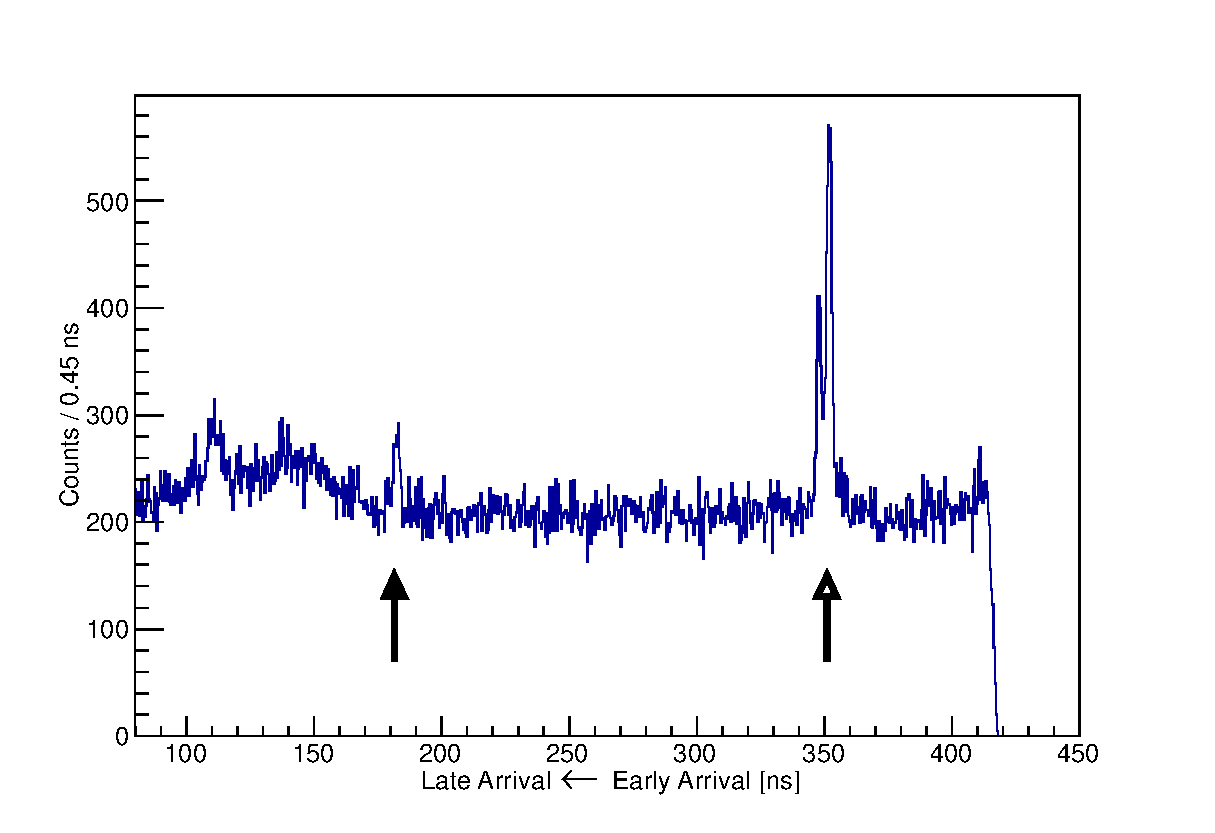
\includegraphics[width=0.5\textwidth]{figures/74Ge_sep_PS_barA.eps}
}
\subfloat[][]{
   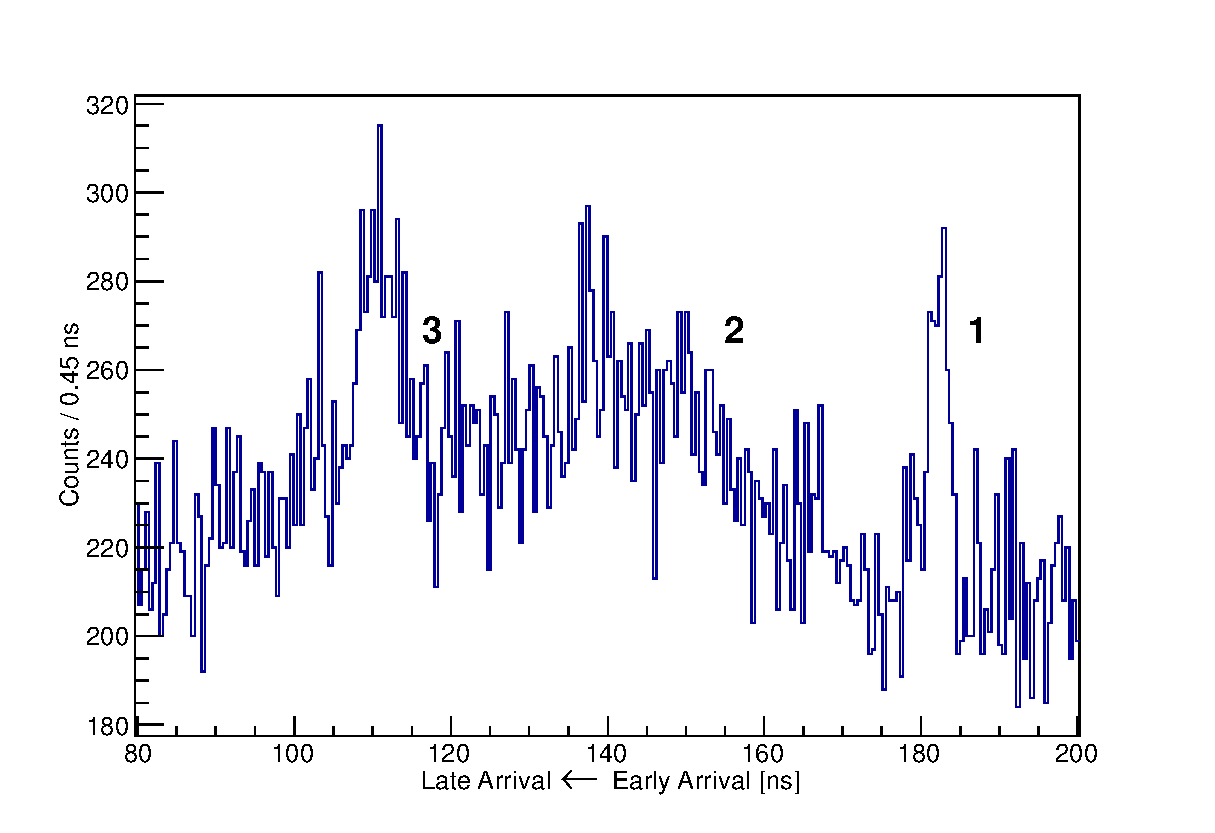
\includegraphics[width=0.5\textwidth]{figures/74Ge_sep_PS_barA_zoom.eps}
}
\caption[Timing spectrum due to $^{74}$Ge($^3$He,n)$^{76}$Se.]{(a) A (time of flight) (TOF) spectrum from the forwardmost neutron detector bar (6.1$^{\circ}$) in the case of pulse-selected beam.  The reaction is $^{74}$Ge($^3$He,n)$^{76}$Se.  The ground-state neutron peak is indicated with a solid arrow and the $\gamma$ peak with a hollow arrow.  Note that the $\gamma$ peak is doubly peaked, from beam hitting the target and then the beamstop.  (b) The neutron TOF spectrum in the region of interest.  The ground-state neutron peak is indicated with a ``1'', the neutron continuum with a ``2''.  The other prominent peak, labeled ``3'', is due to oxygen contamination in the target.}
\label{fig:time}
\end{figure}

% a basic discussion of the data:
% TOF spectrum explained
% energy estimator

\section{Detector Efficiency}
\begin{comment}
deuterium, Mg, cuts
\end{comment}
\label{sec:efficiency}
The number of counts due to neutrons measured by the detector scales linearly with the absolute cross section of \reaction but must be corrected for the fact that not all the neutrons leave a signal in the detector.  The ratio of the detected neutron flux to the total neutron flux is called the efficiency of the detector and must be carefully determined as its error contributes directly to the systematic uncertainty of the extracted absolute cross sections.

The efficiency of a plastic-scintillator-type neutron detector depends not only on the energy of the neutron, but also on the detector's size, shape, energy resolution, and detection threshold.  A Monte-Carlo code developed by Cecil \citep{Cecil_neutEfficiency} calculates the efficiency of plastic scintillator detectors for a wide range of neutron energies and detector thresholds to within 10\%.  The Cecil code was used to calculate efficiencies of the neutron detector for neutrons with energies of 10-28~MeV.  The efficiencies predicted by the Cecil code were verified against d(d,n) and \MgReaction measurements, both of which have well-known cross sections.  Comparing the calculated efficiency to measured efficiency over a range inclusive of the neutron energies produced in \reaction gives confidence that the code accurately models the detector.   The inputs required by the code are the density of the detector, its hydrogen to carbon ratio, the energy threshold applied to the data, and the interval over which the detector averages the light output, i.e., the resolution of the detector.  The plastic properties are reported in {\tab}~\ref{tab:WLS_Kuraray}, and the threshold and resolution of the detector must be determined from the energy spectrum of the selected events from the experiment.  The cuts applied to the data are discussed in {\sect}~\ref{sec:cuts}.  An energy spectrum of the ground-state neutrons of any of the reactions studied can be produced by gating on the ground-state peak in the TOF spectrum.  The energy spectrum for the ground-state neutrons from \MgReaction is shown in {\fig}~\ref{fig:lowEnergyCut}.  The width of the high-energy falloff gives the resolution of the detector, and the threshold can be determined by assuming the scale has a zero offset.  That this is a reasonable assumption is confirmed by the accuracy of the calculation.

\begin{figure}[hp]
\centering
\includegraphics[width=0.8\textwidth]{figures/Lite_28MeV.eps}
\caption[Total light deposited 28-MeV neutrons.]{The light curve for 28-MeV neutrons from \MgReaction is obtained by restricting the events to those in the ground-state peak window.  The data points (red, shaded circles) are from the January dataset.}
\label{fig:lowEnergyCut}
\end{figure}
  
The efficiencies calculated using the above method must be checked for absolute accuracy of the prediction as well as accuracy of its predicted dependence on the energy of the detected neutron.  The reaction d(d,n), measured at beam energies near 9~MeV \citep{deuteronCrossSections}, produces ground-state neutrons and is particularly useful because the neutron energy changes drastically as a function of angle, making it a useful check on the energy dependence of the Cecil prediction.  Additionally, empirical fits as described in {\refref}~\citep{deuteronCrossSections} provide excellent estimates of the absolute cross section in this energy region.  The agreement is excellent, as can be seen in {\fig}~\ref{fig:DeuteriumMatch}, which shows the prediction with and without correcting for neutron energy.  This result suggests that the Cecil code accurately adjusts the detector efficiency for neutron energy.  

\begin{figure}[hp]
\centering
\includegraphics[width=0.8\textwidth]{figures/deuteriumMatch.eps}
\caption[Matching the detector efficiency with d(d,n).]{The prediction for d(d,n) (solid line) matches the data well when the efficiency is corrected for the neutron energy (red, shaded circles).  The green, square points represent the differential cross section where the efficiency is assumed to remain constant despite a changing neutron energy.}
\label{fig:DeuteriumMatch}
\end{figure}

That the Cecil code appears to be successful in calculating the efficiency of the neutron detector for 12-MeV neutrons is encouraging, but neutrons from the ground states of \reaction will be $\sim$26~MeV.  A reaction with measurements of cross sections for neutron energies in this range is \MgReaction.  While this reaction has not been measured at the beam energy of 16~MeV, which would produce a $\sim$28-MeV ground-state neutron, it has been measured at lower and higher energies \citep{MgCrossSection1,Bohne_Mg} as shown in {\fig}~\ref{fig:efficiencyCalib}.  The efficiency measured for the neutrons from this reaction provides a measurement very near the $\sim$26-MeV neutrons produced in \reaction and can be used to verify the absolute efficiency predicted by the Cecil code at neutron energies relevant to \reaction.  {\fig}~\ref{fig:efficiencyCalib} shows the consistency of the measured cross section using that predicted efficiency.  While the agreement between measured cross-sections suggests a systematic error due to efficiency of less than 10\%, the estimated systematic error of the data from \MgReaction is $\sim$20\% \citep{MgCrossSection1,Bohne_Mg} and does not provide a better bound than the error associated with the Cecil code.

\begin{figure}[hp]
\centering
\includegraphics[width=0.8\textwidth]{figures/magnesiumMatch.eps}
\caption[Checking consistency of efficiency calculation with \MgReaction by comparing to nearby measured cross sections.]{Checking consistency of efficiency calculation with \MgReaction.  Black squares show previous experimentally-measured values of the cross section.  This work (green triangles) is consistent with calculations.  The calculations (red circles) are coupled-channel DWBA calculations following the prescription of \citep{MgCrossSection1}.  The blue lines indicate the estimated systematic error of the calculation.  The systematic error of the data produced in this work is not shown, while the systematic error of the other data points is shown.  The experimental systematic error of the zero-degree cross section of \MgReaction is approximately 10\%, due primarily to the detection efficiency.}
% circles - CCBA
% blue lines estimate of systematic error due to CCBA parameters
% squares are existing data
\label{fig:efficiencyCalib}
\end{figure}
\FloatBarrier

\section{Experimental Parameters Related to the Cross Section}
\begin{comment}
current, tgt thickness (RBS), solid angle, dead time
go ahead and discuss errors while you discuss these quantities
\end{comment}

The differential cross section is the number of times a reaction occurred ($N_{\text{reaction}}$) normalized by the total number of particles incident on the target ($N_{\text{beam}}$), the number density of nuclei in the target ($n_{\text{target}}$), and the {efficiency of the detector}~($\epsilon$):
\begin{align}
\frac{d\sigma}{d\Omega} &= \frac{N_{\text{reaction}}}{N_{\text{beam}} \times n_{\text{target}} \times \epsilon}.
\label{eq:cross_section}
\end{align}
The efficiency $\epsilon$ of the detector includes the solid angle $d\Omega$.  Other quantities in the cross section that relate to the experimental setup are the number of particles incident on the target and the number density of nuclei in the target.

The three targets (\GeTargets and \Mg{26}) used in the experiments were provided by John Greene of Argonne National Laboratory (ANL).  The \GeTargets targets were evaporated onto a gold backing, while the \Mg{26} target is self-supporting.  The isotopic abundance and thickness of each target is shown in {\tab}~\ref{tab:targets}.  The target thicknesses were measured with an alpha-thickness gauge when they were made, and again at Hope College using Rutherford back-scattering (RBS).  RBS measurements are useful because they give information about the target composition, which must be assumed when calculating target thickness from alpha-thickness-gauge measurements.  The reported thicknesses were obtained by analyzing the RBS data with SIMNRA \citep{SIMNRA}, an RBS analysis software.  A sample of the fit for each target is shown in {\fig}~\ref{fig:RBS_sample}.  Measurements taken at several different positions on each target showed that variations in target thickness were approximately 1\%.  The predominant features of the RBS spectrum are the plateaus due to the germanium layer and the gold foil.  These plateaus overlap, but the features due to beam scattering from the front and back surface of each layer are clearly visible.  {\fig}~\ref{fig:RBS} and {\fig}~\ref{fig:rawDataRBS} identify these features.  This RBS spectrum also shows evidence of small pinholes in the target; they introduce a low-energy aluminum spectrum that is highlighted in red in {\fig}~\ref{fig:RBS}.  There are also small areas of the target that are bare gold foil, evidenced by the very small plateau at high energies that is highlighted in green.  These features do not alter the estimate of the target thickness, which depends only on the edges of the plateau.  Because the edges of the plateau are well defined, the uncertainty in the number of target atoms is less than a percent.  A cautious estimate of the uncertainty in the cross section due to the target is 2\%.  A fit to the data adjusted for the pinholes is shown in {\fig}~\ref{fig:RBS_sample}.

To determine the absolute cross section, it is also necessary to know the total number of \He{3} ions incident on the target for each dataset.  One monitor of the beam current is the charge collected by the Faraday cup.  A BaF$_2$ crystal outside the target chamber and a silicon detector inside the target chamber detect $\gamma$ radiation from beam incident on the target and scattered \He{3} beam, respectively.  Both these detectors monitor the product of the target thickness and the beam current.  Data from the silicon detector show that the ratio of \GeTargets to gold does not change throughout the run, demonstrating that the targets are stable throughout the run.  Additionally, the back-scattered peak in the silicon spectrum scaled with the live charge, which is the charge scalar vetoed by the DAQ busy as discussed in {\sect}~\ref{sec:electronics}.  The live charge can therefore be used to scale beam current between runs, making it possible to express \reaction cross sections in terms of the known \MgReaction cross section.

\begin{figure}[hp]
\centering
\subfloat[][]{
   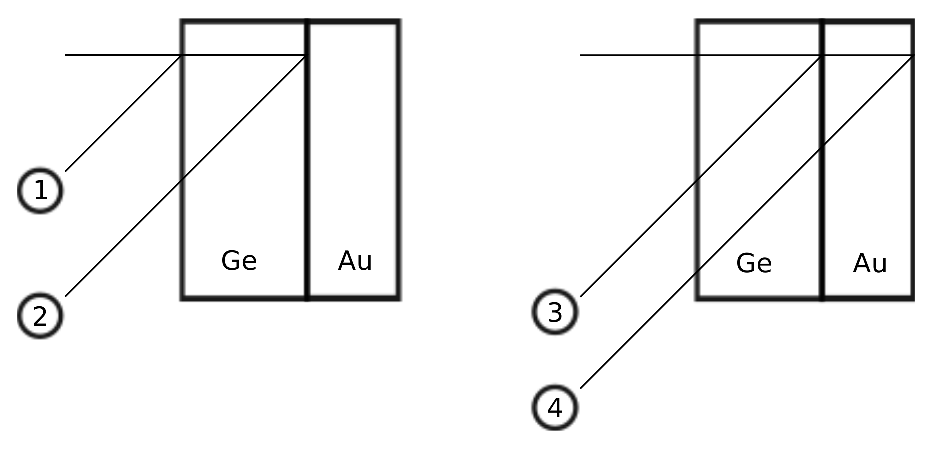
\includegraphics[width=0.5\textwidth]{figures/RBS_possibilities.eps}
   \label{fig:RBS}
}
\subfloat[][]{
   \includegraphics[width=0.5\textwidth]{figures/76ge-4-holes.eps}
   \label{fig:rawDataRBS}
}
\\
\subfloat[][]{
   \includegraphics[width=0.8\textwidth]{figures/76ge-4-adjusted.eps}
   \label{fig:RBS_sample}
}
\caption[Interpreting RBS data and constraining the target thickness.]{\subref{fig:RBS} Beam scattering from the front and back layer determines the high and low energy plateau edges.  The scattering angle is shown as forward to compress the figure but was backward at 168$^\circ$ in the experiment.  \subref{fig:rawDataRBS} RBS data for the \Ge{76} target near the beamspot.  The features used to determine the thicknesses of the gold and germanium layers are marked.  \subref{fig:RBS_sample} The RBS spectrum, adjusted by subtracting the background due to pinholes, and its fit.  Fitting the RBS spectrum with and without adjusting for pinholes did not result in any significant differences to the predicted target composition or thickness.}
\end{figure}

\begin{table}[hp]
\ra{1.1}
\centering
\caption[\uppercase{target composition and thickness}]{\\\uppercase{target composition and thickness}}
\label{tab:targets}
\begin{tabular}{lllll}\toprule
 & \multicolumn{2}{c}{$\alpha$-gauge ($\mu$g/cm$^2$)} & \multicolumn{2}{c}{RBS ($\mu$g/cm$^2$)} \\
\cmidrule(r){2-5}
$^{74}$Ge (98.9\%) & Au$_{\text{nat}}$ & 1011 & Au$_{\text{nat}}$ & 1001 \\
          & $^{74}$Ge & 1057 & $^{74}$Ge & 1016 \\
          &           &      & O$_{\text{nat}}$ & 9 \\[0.35cm]

$^{76}$Ge (92.82\%) & Au$_{\text{nat}}$ & 1069 & Au$_{\text{nat}}$ & 1014 \\
          & $^{76}$Ge & 838 & $^{76}$Ge & 775 \\
          &           &      & O$_{\text{nat}}$ & 4 \\[0.35cm]

$^{26}$Mg ($>$99.55\%) & $^{26}$Mg & 791 & $^{26}$Mg & 685 \\
          &           &      & C$_{\text{nat}}$ & 10 \\
          &           &      & N$_{\text{nat}}$ & 43 \\
          &           &      & O$_{\text{nat}}$ & 52 \\
\bottomrule
\end{tabular}
\begin{flushleft}
{\footnotesize NOTE:
Target composition and thickness.  The isotopic abundance of the target is listed in parenthesis.  The $\alpha$-gauge measurements were performed at ANL and the RBS measurements at Hope College.}
\end{flushleft}
\end{table}
\FloatBarrier


\section{Data Sets}
Two sets of \reaction data are available.  The first was taken in September 2011.  A subset of this data was taken with no pulse selection due to hardware failure.  A second run in January 2012 provided additional data, all taken with pulse selection.  During the January run, data were taken with the \GeTargets as well as \Mg{26} targets to provide an accurate normalization.  The data sets are summarized in {\tab}~\ref{tab:dataSets}.  While the non-pulse-selected data was useful in constraining parts of the pulse-selected background (see {\sect}~\ref{sec:PS_data}), it was not possible to estimate the background well enough to obtain useful cross-section data from these runs.  Thus, the non-pulse-selected data appear in this chapter only as a constraint on a fit to the pulse-selected data.

\begin{table}[hp]
\ra{1.1}
\centering
\caption[\uppercase{data sets}]{\\\uppercase{data sets}}
\label{tab:dataSets}
\begin{tabular}{llll}\toprule
            & & Live Time (s) & Live Charge ($\mu$C)\\
\cmidrule(r){3-4}
January     & PS \Mg{26} & 46460 & 1044 \\
	    & PS \Ge{76} & 78140 & 2919 \\
	    & PS \Ge{74} & 163800 & 5313 \\ \\

September   & PS \Ge{76} & 126200 & 2873 \\
	    & PS \Ge{74} & 116700 & 2619 \\
	    & NPS \Ge{76} & 273700 & 15320 \\
	    & NPS \Ge{74} & 113200 & 10010 \\
\bottomrule
\end{tabular}
\begin{flushleft}
{\footnotesize NOTE:
Data sets used in the analysis were obtained in two separate runs.  Both pulse-selected (PS) and non-pulse-selected (NPS) data were taken during the September run.}
\end{flushleft}
\end{table}
\FloatBarrier

\section{Cuts}
\label{sec:cuts}
Four sets of cuts were applied to the data to generate a final data set.  The first cut verifies that the recorded event represents a real event rather than noise.  The next cut discards events with too-low light signals, reducing the background due to $\gamma$ radiation.  Two final cuts reduce the muon background; one cut uses the veto, and the other eliminates events with light signals too large to be due to neutrons.

A true event should have energy above the noise level recorded in both top and bottom PMT's.  Additionally, the time signals from the top and bottom PMT's should be correlated.  A typical scatter plot of timing from the top and bottom PMT are shown in {\fig}~\ref{fig:realEvent}.  Requiring correlated top and bottom timing signals is a cut that is applied to all bars in all final data sets.  The other requirement for a valid event is that the light signal be above the noise threshold.  An example of a light spectrum for a single bar is shown with the noise threshold already applied {\fig}~\ref{fig:realEvent}.

\begin{figure}[hp]
\centering
\subfloat[][]{
  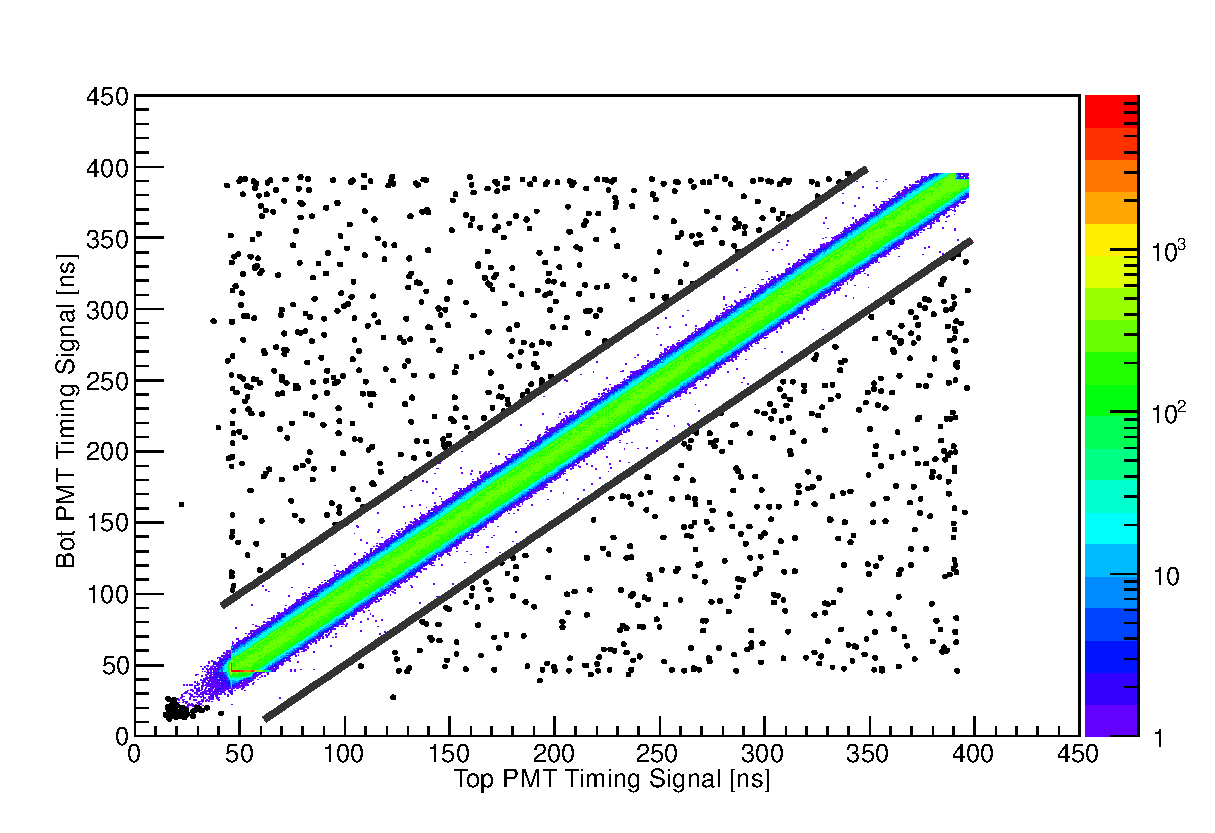
\includegraphics[width=0.8\textwidth]{figures/realTiming.eps}
}\\
\subfloat[][]{
  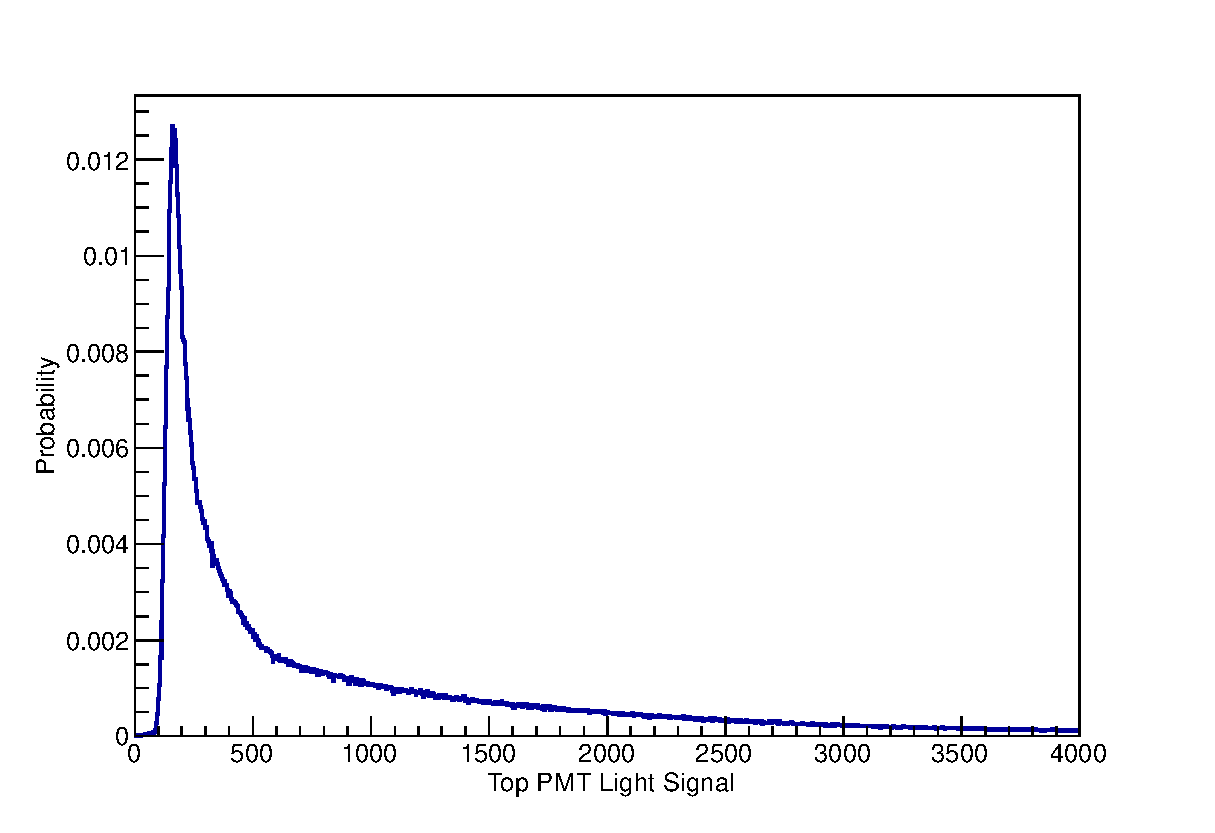
\includegraphics[width=0.8\textwidth]{figures/lightThreshold.eps}
}
\caption[Cuts used to determine event validity include timing correlation and a light signal above the noise threshold.]{(a) For a real event, the timing signal from a bar's top and bottom PMT will be similar.  Times differing by more than 100 ns are rejected.  Events with correlated timing are shown in color and are inside the thick gray lines.  The larger, black dots indicate events whose timing is not considered correlated.  (b) A low noise threshold placed on the PMT signal discards spurious events.}
\label{fig:realEvent}
\end{figure}

% discussion of muon rejection begins here
Both the veto paddles and the bars of the neutron detector serve as a veto.  Veto paddle information is recorded as either ``true'' or ``false'' - true if a veto paddle fired during the event, false if it did not.  The bars of the neutron detector, in contrast, have more detailed information - time and light output.  While accidental coincidences are rare, this additional information is used when a neutron bar is used as veto material.  For one bar of the neutron detector to veto another, both must have a valid signal and their average time must be similar.

A first approximation to determining whether or not an event is the result of a muon interaction is to require all but one bar in the neutron detector, as well as the entire veto, to be silent.  However, this would veto events that are spatially disconnected and could not possibly be due to a single muon.  To eliminate these unnecessary vetoes, we look at events that register signals in detectors with close spatial proximity, a ``veto group''.  One way to determine the appropriateness of increasing the size of a veto group is by looking at the energy spectrum of vetoed events.  Adding detectors to a veto group that primarily eliminates muons results in an energy spectrum that has roughly equal numbers of high and low energy events, as shown in {\fig}~\ref{fig:muonVetoSpectrum}.  Material that does not veto primarily muon events will yield an energy spectrum that appears much more like the room background spectrum, heavily weighted towards lower energy events, as in {\fig}~\ref{fig:notMuonVetoSpectrum}.  These figures indicate that an appropriate group of material to use in the veto of a detector bar is the immediate, surrounding material.  Several samples of veto groups are shown in {\fig}~\ref{fig:vetoGroups}.  A separate cut to reject muons discards events that deposit energy above the maximum neutron energy deposition.

\begin{figure}[hp]
\centering
\subfloat[][]{
   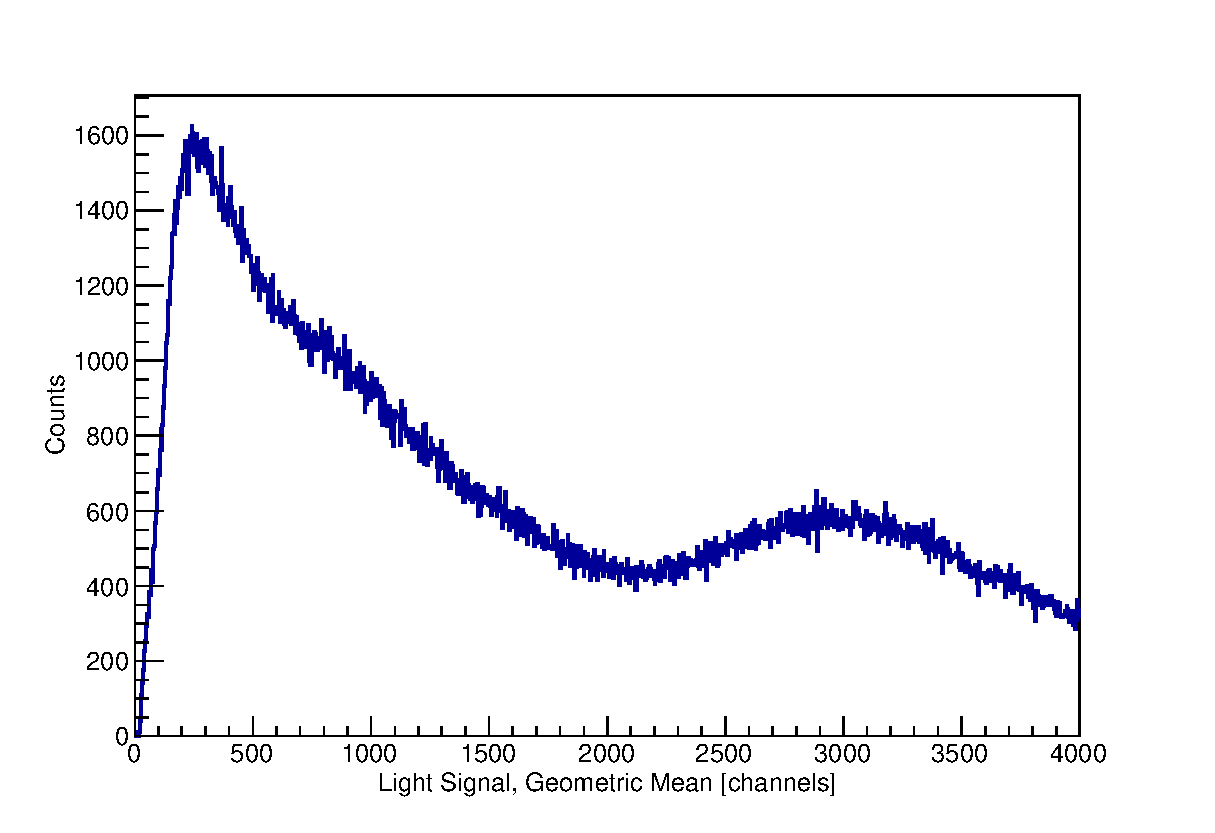
\includegraphics[width=0.45\textwidth]{figures/atLeastOneCorrelatedBar.eps}
   \label{fig:muonVetoSpectrum}
}
\hspace{8pt}
\subfloat[][]{
   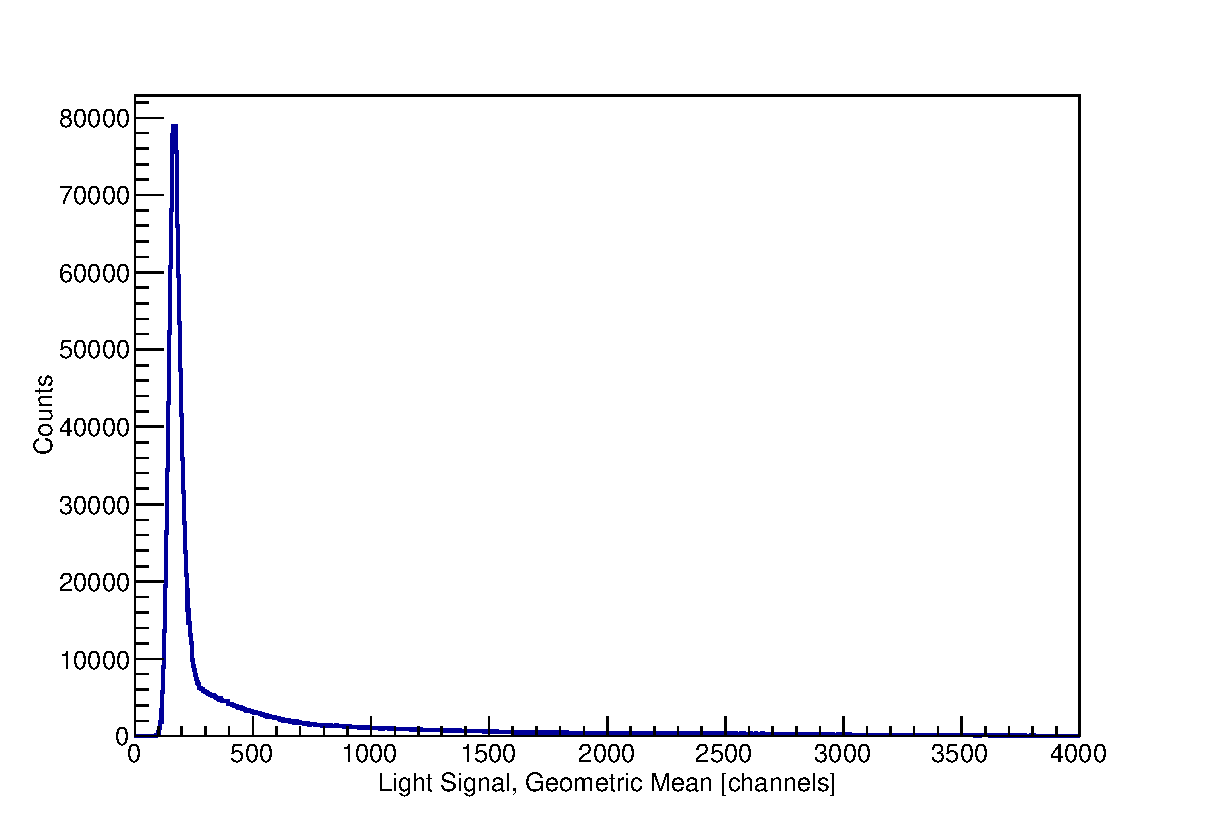
\includegraphics[width=0.45\textwidth]{figures/singleBar_noVeto.eps}
   \label{fig:notMuonVetoSpectrum}
} \\
\subfloat[][]{
   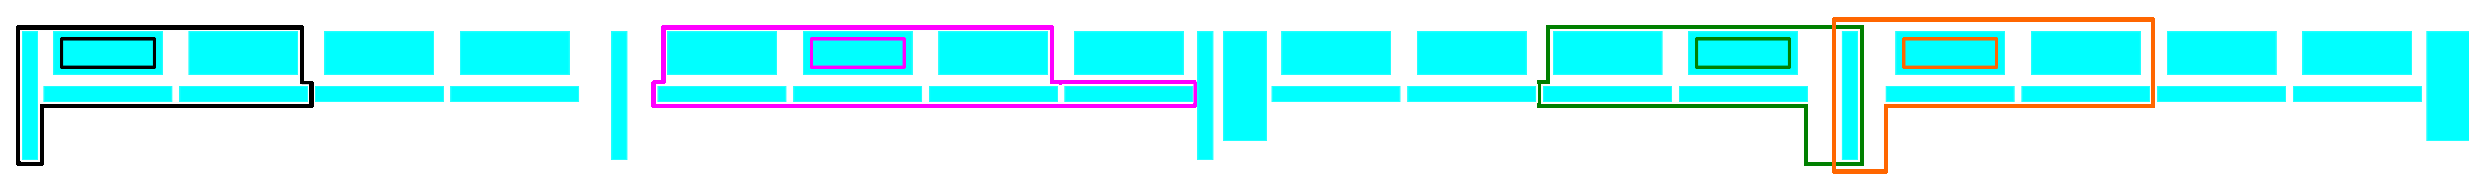
\includegraphics[width=1.0\textwidth]{figures/vetoGroups.eps}
   \label{fig:vetoGroups}
}
\caption[Determining appropriate groups of detectors for vetoing by examining the vetoed energy spectrum.]{(a) Energy spectrum of a neutron detector bar.  Entries in this histogram are from events having at least one correlated signal in the neutron detector and are likely to be muons.  Notice the high-energy-deposition peak at $\sim$ channel~3000 and its considerable height relative to the low-energy $\gamma$ background.  This low-energy background is dominant in non-muon events as in {\fig}~\subref{fig:notMuonVetoSpectrum}.  (b) Neutron detector bar energy spectrum.  These events have no correlation to other signals in the neutron detector and are unlikely to be due to muons.  While some high-energy depositions are visible, the spectrum is clearly dominated by the low-energy peak due to $\gamma$ radiation.  (c) Sample groups of detectors chosen to veto bars in the neutron detector.  If the events in a neutron detector bar vetoed by a detector have an energy spectrum dominated by the low-energy $\gamma$ radiation, that detector is not used as part of the veto for that particular bar.}
\label{fig:determineVetoGroups}
\end{figure}

% discussion of the low energy cut begins here
The final cut on the data sets is a lower-energy cut to reduce the random background due to $\gamma$ radiation.  Placing a low-energy cut on the data is difficult because finding an estimator for the energy is not straightforward.  It is appealing to argue that light loss due to attenuation must be exponential, and that an accurate estimator of the total deposited energy is the geometric mean of the top and bottom PMT signals:
\begin{equation}
\sqrt{Ae^{-\alpha x}\times Ae^{-\alpha (L-x)}} = \sqrt{A^2e^{-\alpha L}} = Ae^{-\alpha L/2},
\end{equation}
where $\alpha$ is a factor determined by the attenuation in the bar and $L$ is its length.  If this model of the signal attenuation is correct, the geometric mean should be position-independent.  This is not the case, as can be seen in {\fig}~\ref{fig:product_positionDependence}.  Furthermore, the position dependence is not often uniform even between the top and bottom PMT on a single bar, making it difficult to construct an average value.  It is necessary to define a low-signal cut that is uniform for all the bars of the detector because the efficiency is sensitive to the low-energy threshold.  Determining a threshold that is uniform from bar to bar is therefore necessary to avoid introducing significant error into the extracted ground-state counts.

\begin{figure}[hp]
\centering
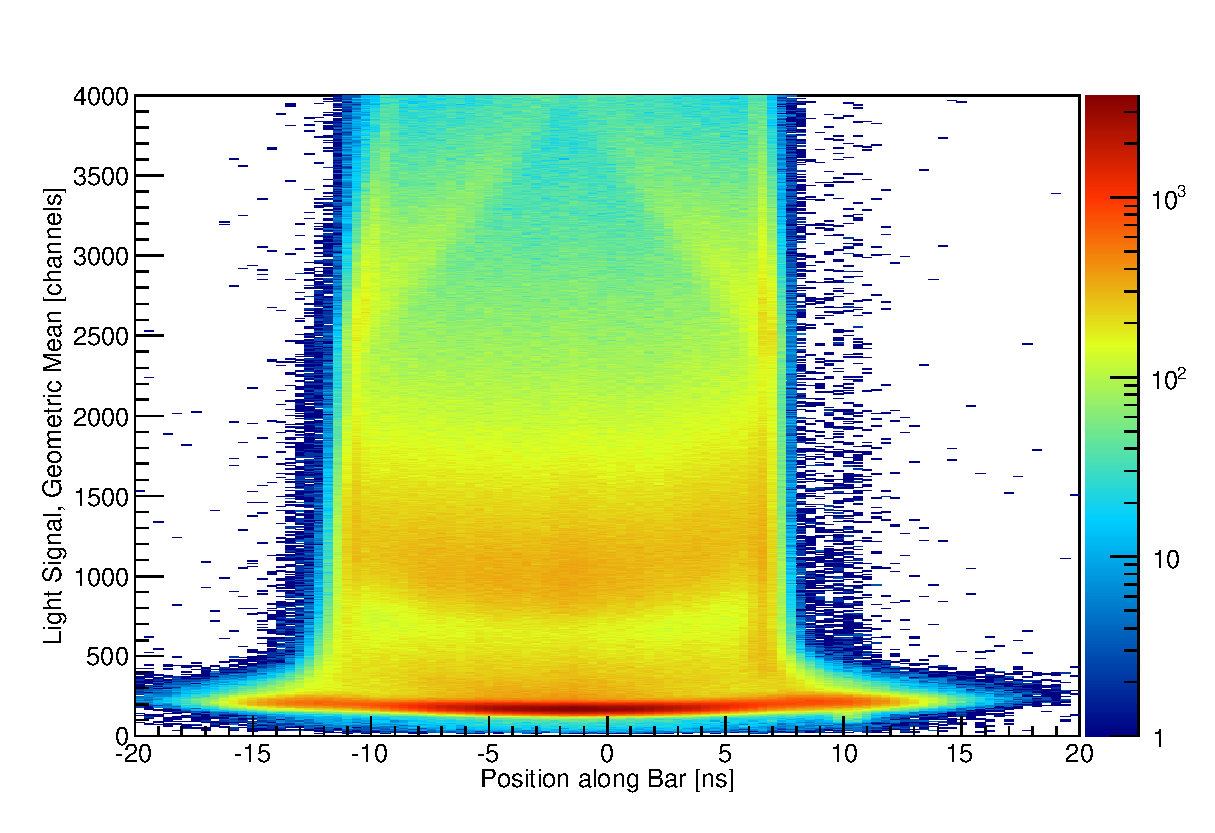
\includegraphics[width=0.8\textwidth]{figures/positionVSenergy.eps}
\caption[Position dependence of the geometric mean of the light signal of rejected events.]{Position dependence of the geometric mean of the light signal of rejected events.  The band of events with light signals between $\sim$1000-1500~channels in particular demonstrates that the signal increases as it approaches the extremes of the neutron detector bar.  The events shown here are those that triggered the veto and are likely muons.}
\label{fig:product_positionDependence}
\end{figure}

Defining a position-dependent light signal cut on each PMT separately would be an ideal solution to these problems if the position dependence for a given energy deposition were known.  While such a characterization of the detectors for an arbitrary energy is not known, the muon veto provides a single calibration point by allowing the extraction of a data set that is predominently muon events.  Due to the detector geometry, it is expected that the average path of the muons will be peaked at slightly more than 5~cm.  Simulations using the detector bar geometry and an angular distribution of $\cos^{2.4}{\theta}$ \citep{cosmicsZenithDependence} (where $\theta$ is the zenith angle) confirm a well-defined peak in the muon path length. This most-likely path length of the incident muons manifests as a peak in the energy spectrum that depends only on the thickness of the bar and on the most likely angle of the trajectory because the muons are MIP's.  Note that both the bar thickness and the most likely angle of a muon path are the same for every bar in the neutron wall.  In addition, the thickness of the neutron detector bars places this peak well above the thorium edge, at approximately 15~MeVee.  A simulated energy spectrum is shown next to a real energy spectrum in {\fig}~\ref{fig:muonSpectrum}.  The peak of the light spectrum is assumed to represent the same energy and therefore to function as a calibration of the position dependence of the light signal due to the most likely muon energy deposition.  Fits to the location of the energy peak as a function of position are shown in {\fig}~\ref{fig:fits_pkVSpos}.

\begin{figure}[hp]
\centering
\subfloat[][]{
   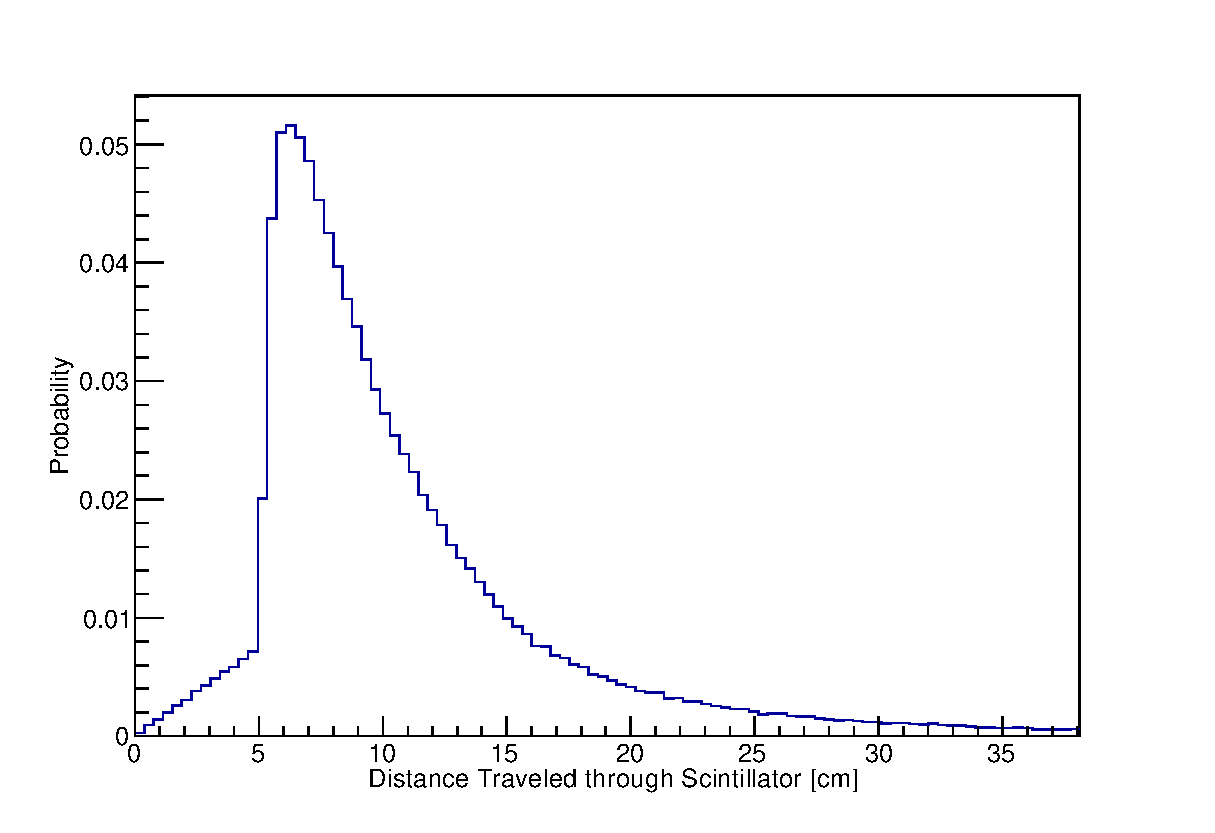
\includegraphics[width=0.5\textwidth]{figures/cosDist_distances.eps}
}
\subfloat[][]{
   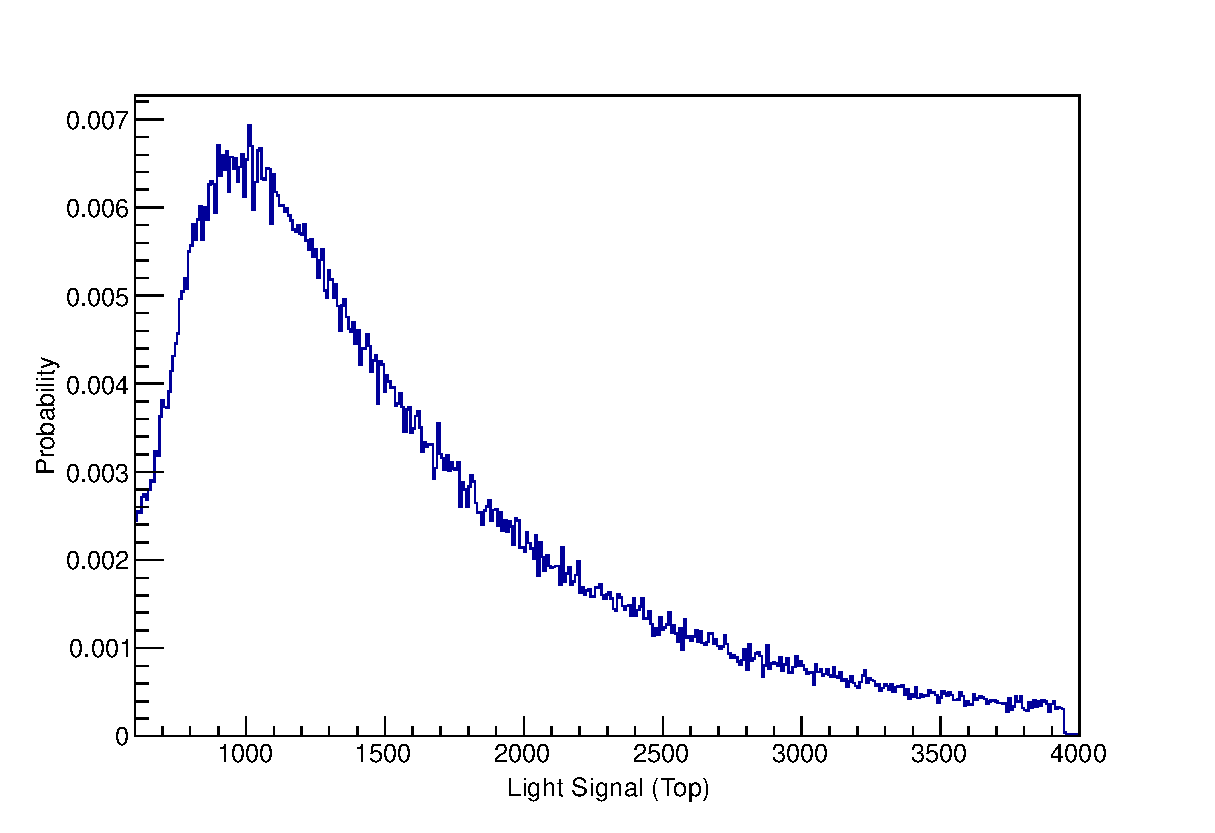
\includegraphics[width=0.5\textwidth]{figures/BarA_cosmics_centerSlice.eps}
}
\caption[Characteristic peak in energy spectrum due to muons.]{(a) A simulation of path length of muons interacting in a detector with dimensions identical to those of the neutron detector bars.  All muons are assumed to be MIP's, which implies that distance traveled in the scintillator linearly transforms into energy deposited in the scintillator.  Note the distinct peak. (b) Light signal of muon events near the center of the bar.  The peak in this distribution is believed to be the peak seen in the simulated spectrum.}
\label{fig:muonSpectrum}
\end{figure}
% new figure
\begin{figure}[hp]
\centering
\subfloat[][]{
   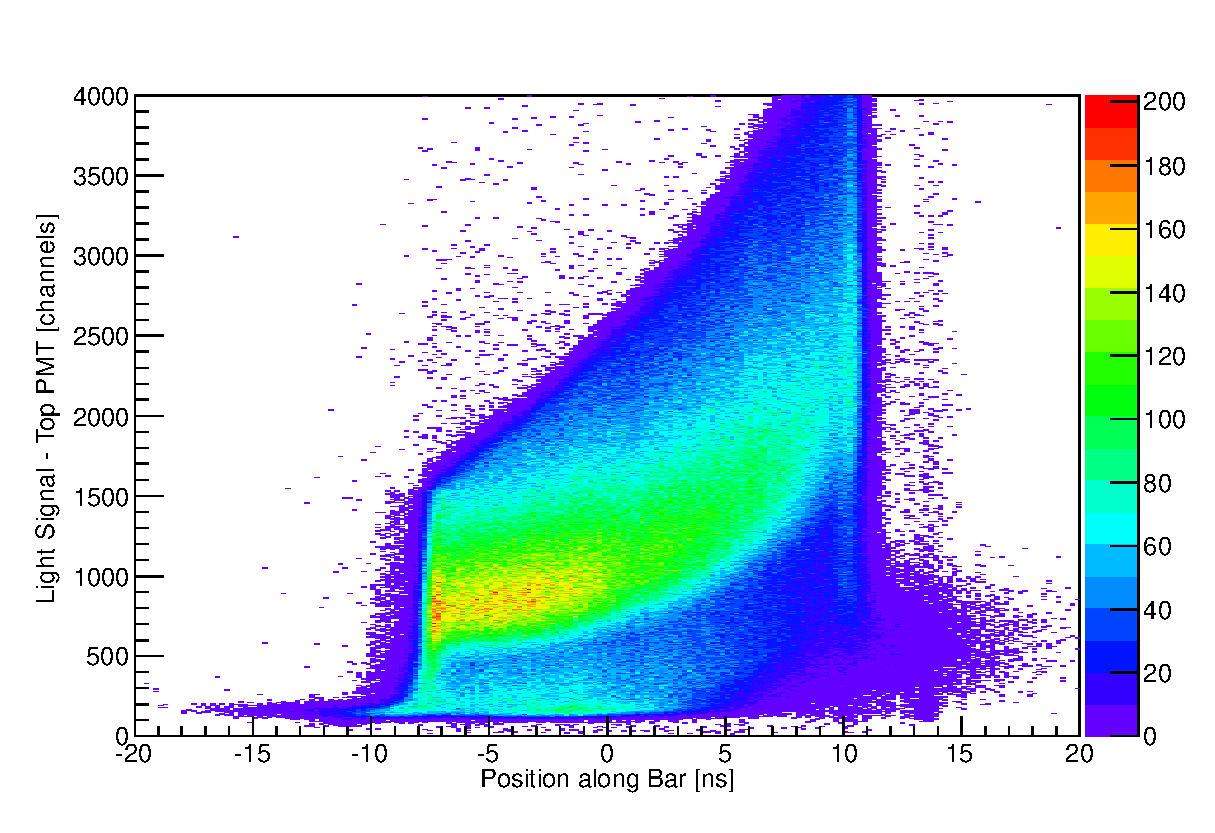
\includegraphics[width=0.8\textwidth]{figures/PMT_positionResponse.eps}
} \\
\subfloat[][]{
   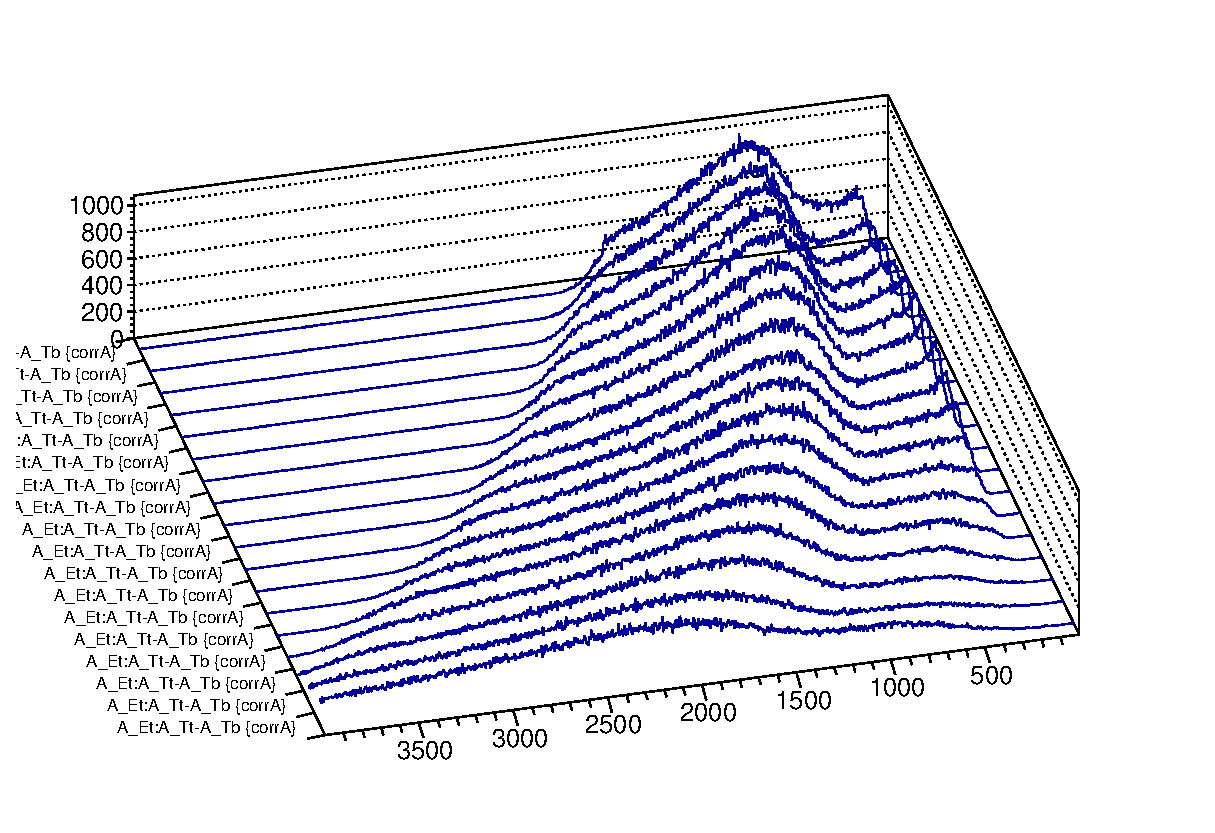
\includegraphics[width=0.45\textwidth]{figures/position_sliceGraphs.eps}
}
\hspace{8pt}
\subfloat[][]{
   \includegraphics[width=0.45\textwidth]{figures/EnergyCutExample.eps}
}
\caption[Determining the position-dependent lower-energy cut using the energy spectrum due to muons.]{(a) The position dependence of the light signal from a single PMT.  (b) The two-dimensional histogram shown in (a) is projected into a series of one-dimensional histograms.  The peaks of these histograms are determined by fitting with a Landau function.  (c) A plot describing the curve which, when scaled, is used as the low-energy cut.  The points are determined from the histograms shown in (b).  Points at the extremes that do not follow the trend are used to determine the position cut.}
\label{fig:fits_pkVSpos}
\end{figure}

Using this ``constant-energy curve'' directly as a lower-energy cut is too high an energy cut as can be seen in {\fig}~\ref{fig:highEnergyCut}.  Instead, a scaling factor is applied to these curves that maximizes the signal to noise ratio; the scaled curves serve as appropriate energy cuts.  While high cuts discard more background, they also discard more neutrons of interest, which can deposit a small amount of energy in the detector.  The minimum fractional error of the extracted ground-state counts is achieved with a scaling factor that results in a reduction of the background by a factor of $\sim$1.4 (with all other cuts applied).  This is the case for every bar in the neutron detector; the fractional error as a function of the energy cut for the forwardmost bar is shown in {\fig}~\ref{fig:signalToNoise}.  Scaling ratios are determined by comparing the background to that of the initial cut to obtain uniform scaling from bar to bar.  
\begin{figure}[hp]
\centering
\subfloat[][]{
   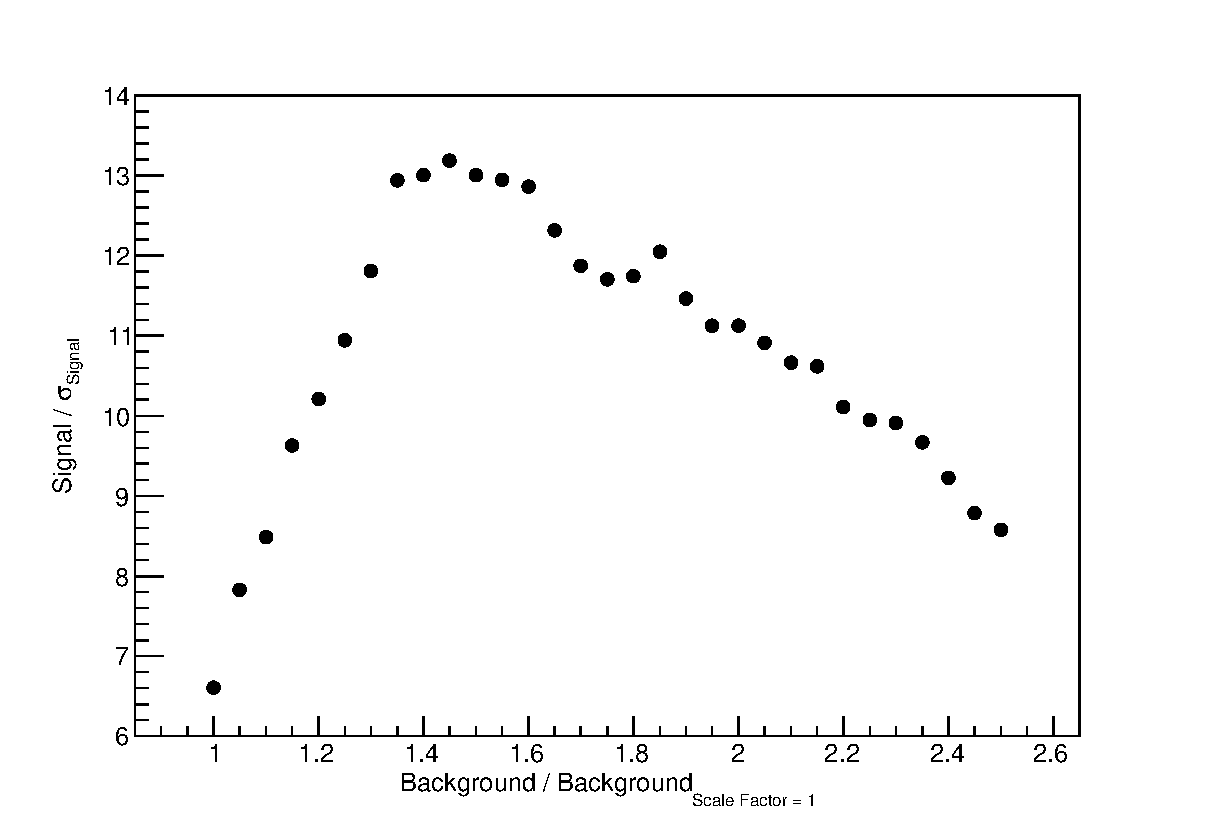
\includegraphics[width=0.45\textwidth]{figures/signalToNoiseCurveA.eps}
   \label{fig:signalToNoise}
}
\hspace{8pt}
\subfloat[][]{
   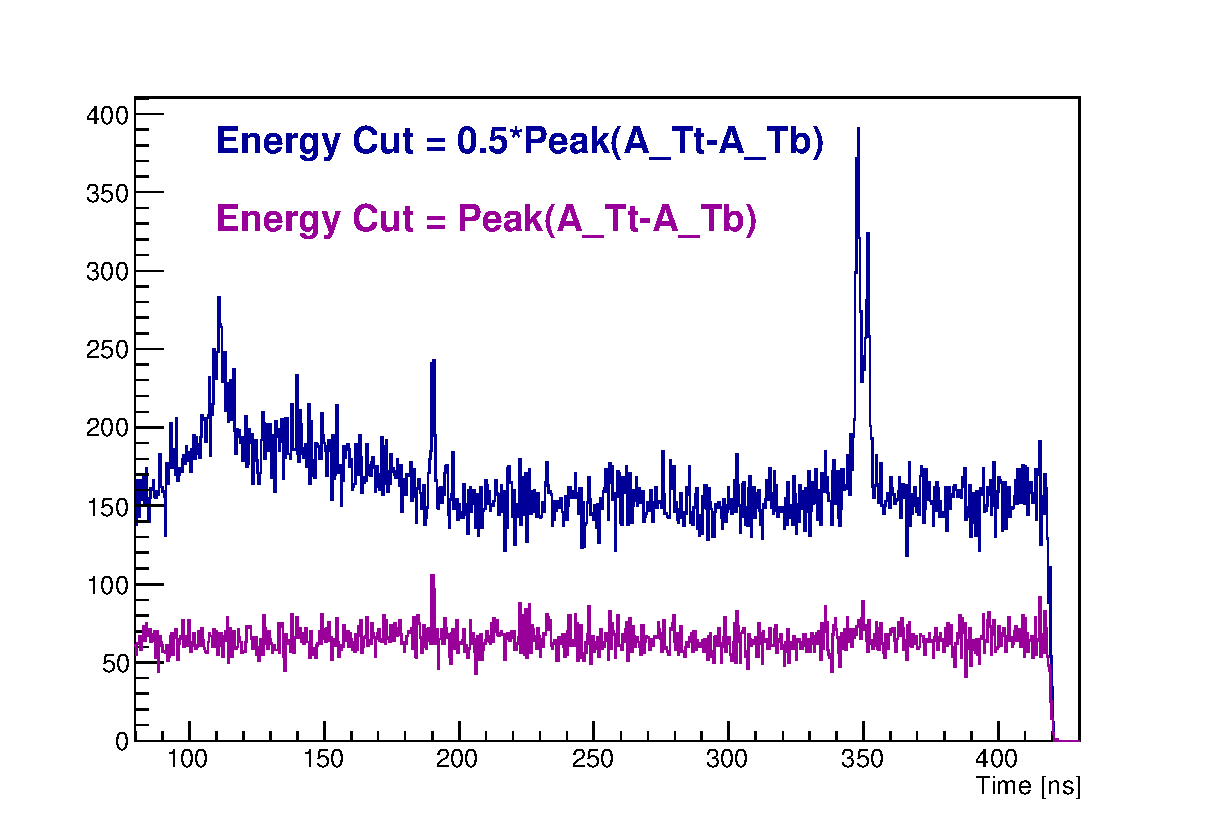
\includegraphics[width=0.45\textwidth]{figures/needLowerCut.eps}
   \label{fig:highEnergyCut}
}
\caption[Optimizing the scale of the low-energy position cut for minimum fractional error.]{(a) The ratio of the signal to its statistical error as a function of the energy cut.  The energy cut is parametrized as the background reduction to allow uniform scaling between bars. (b) Without applying a scaling factor to the cut determined as in {\fig}~\ref{fig:fits_pkVSpos}, the neutron signals are nearly lost.  Scaling the cut by $\sim$0.5 results in a reasonable signal to noise ratio.}
\label{fig:scalingFactorEffect}
\end{figure}

It should be considered that simply scaling the energy cut may not accurately reproduce the position dependence of a smaller deposited energy.  No distinct feature exists at lower energies, making this difficult to check directly.  However, the position distribution of neutron events gives some indication of the accuracy of the position-dependence of the scaled cut.  Because neutrons from the (\He{3},n) reaction should be uniform across a neutron detector bar, an accurate low-energy cut should result in a position spectrum that is approximately flat.  This spectrum, estimated by subtracting the background position spectrum from the position spectrum of events in the timing window of the ground-state neutrons, is shown in {\fig}~\ref{fig:flatPositionSpectrum}.  Its uniformity suggests that the position dependence at the most-likely deposited energy for muons is a reasonable approximation for lower-energy events.

The error associated with the lower-energy cut is non-zero due to the uncertainty associated with the fit to the peak.  An estimate of the error on the extracted signal is
\begin{equation}
\sigma_S^2 = \left( \frac{dS}{dE} \right)^2 \sigma_E^2, 
\end{equation}
where $E$ is a variable denoting the low-energy cut.  The uncertainty $\sigma_E$ is assumed to be the error on the parameter describing the position of the peak of the energy distribution at each position slice (see {\fig}~\ref{fig:fits_pkVSpos}.  The change in number of ground-state counts with respect to the energy cut is determined by numerically estimating the derivative in the region of the chosen energy cut.  For this energy cut, which is approximately one half the maximum deposited neutron energy, the error due to the energy cut is $<$2\%.

\begin{figure}[hp]
\centering
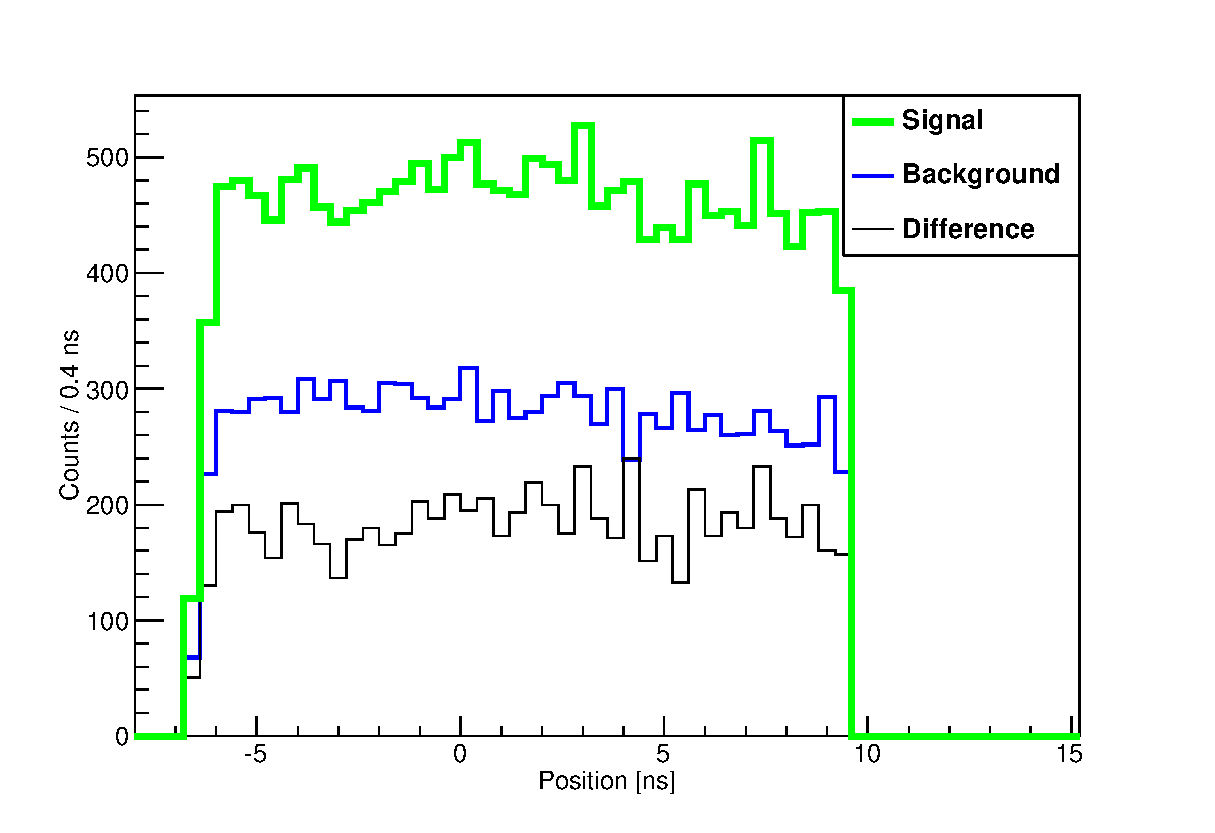
\includegraphics[width=0.8\textwidth]{figures/PositionSpectrum2.eps}
\caption[Testing the validity of the scaled low-energy position cut with position spectra from \MgReaction.]{A histogram of event position with a lower-energy cut based on position.  The data used are the \MgReaction data from January.  The difference between the position spectra of the region around the ground state neutron peak (green) and a background region with the same number of bins (blue) is shown in black.  That this resulting position spectrum is flat indicates that the position dependence of the cut is appropriate.}
% rebin
% make sure spectra are clearly visible
\label{fig:flatPositionSpectrum}
\end{figure}
\FloatBarrier


\section{Ground State Cross-Section}
\begin{comment}
two data sets
- pulse selection
- no pulse selection

background
- gamma peaks - do not overlap with neutron peak
- other neutron peaks - ??
- randoms - background in both data sets
- continuum - more important in non-pulse-selected data

extracting counts 
- pulse selection
- no pulse selection
\end{comment}

To extract the counts due to the ground-state neutrons one can sum the counts in the region of the peak and subtract the estimated background:

\begin{equation}
\text{S = P - B},
\label{eq:counts}
\end{equation}
where S is the extracted number of signal counts, P is the number of counts in the signal region, and B is the number of estimated background counts.  The error associated with $S$ is
\begin{equation}
\sqrt{\sigma_{P}^2 + \sigma_{B}^2}
\label{eq:errDef}
\end{equation}
where both $P$ and $B$ can be understood as a random variable with error $\sqrt{P}$ and $\sqrt{B}$, respectively.

The primary challenge is finding an accurate way to estimate the background that reduces the error of the extracted counts.  As can be seen in {\fig}~\ref{fig:PSvsNPS}, the background of the pulse-selected data is much simpler than that of the non-pulse-selected data.  Without pulse selection, the neutron peak is superimposed on background from previous neutron bunches, making the extracted signal extremely sensitive to poorly-constrained fit parameters.  Only signal estimates from the pulse-selected data are used for the data sets discussed in this thesis.

\begin{figure}[hp]
\centering
\subfloat[][]{
   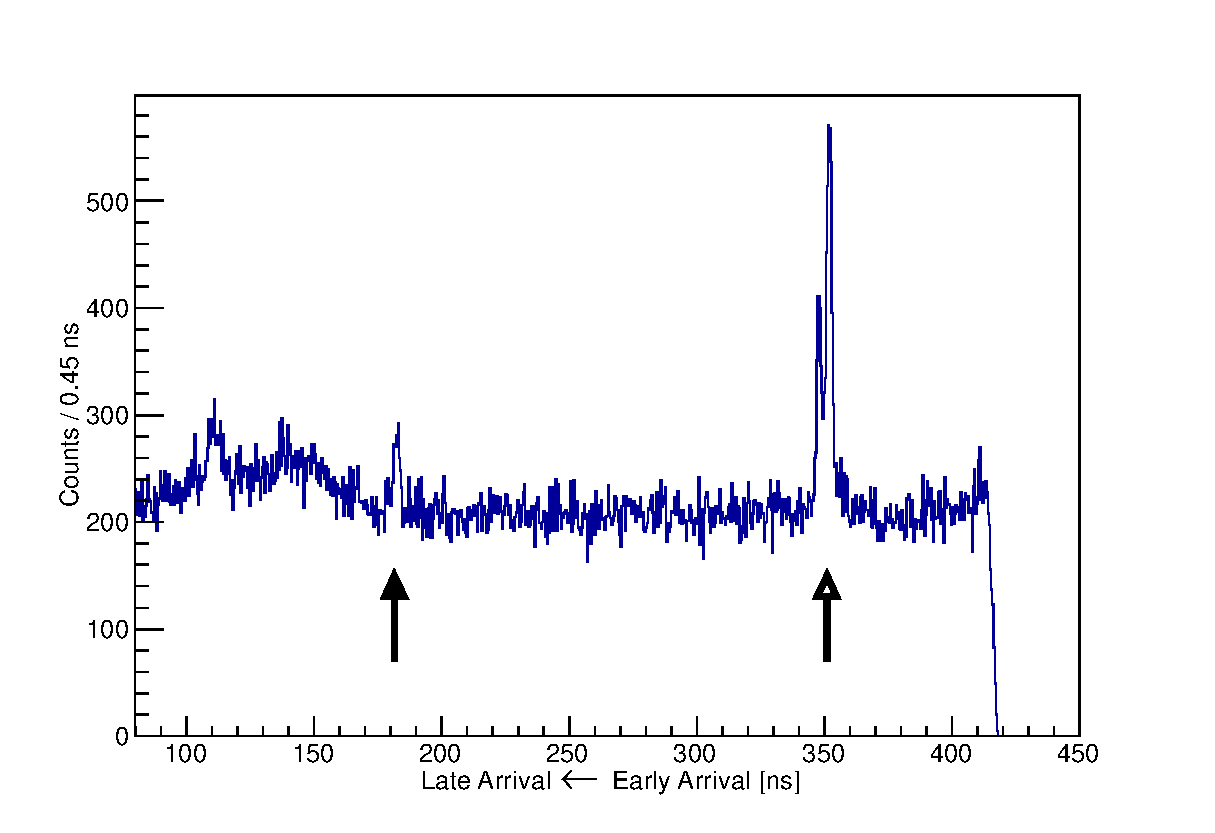
\includegraphics[width=0.5\textwidth]{figures/74Ge_sep_PS_barA.eps}
}
\subfloat[][]{
   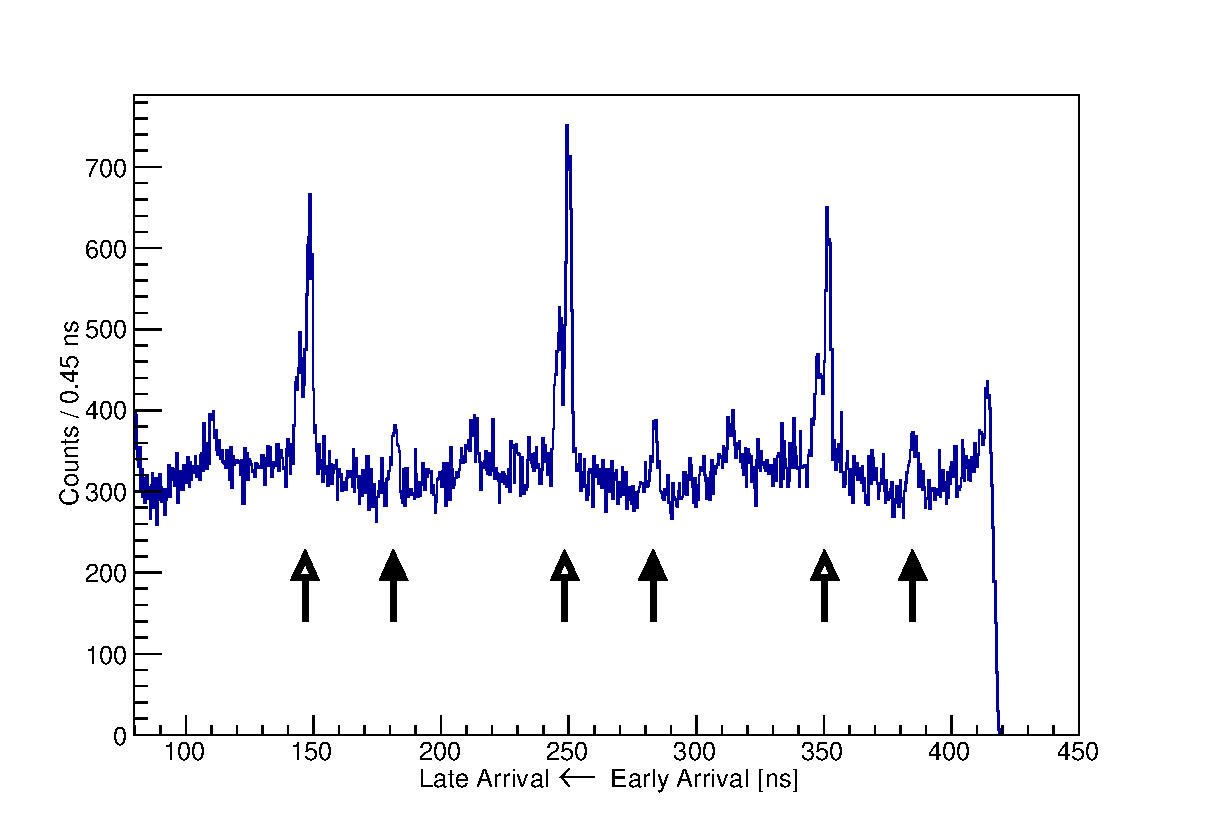
\includegraphics[width=0.5\textwidth]{figures/74Ge_sep_NPS_barA.eps}
}
\caption[Comparison of pulse-selected and non-pulse-selected timing spectra from $^{74}$Mg(\He{3},n).]{(a) The TOF spectrum of the forwardmost neutron detector bar (6.1$^{\circ}$) in the case of pulse-selected beam.  The data is from the September run.  The ground-state neutron peak is indicated with a solid arrow and the $\gamma$ peak with a hollow arrow. (b) The timing spectrum of the  non-pulse-selected beam, also from the September run.}
\label{fig:PSvsNPS}
\end{figure}

\subsection{Pulse-Selected Data}
\label{sec:PS_data}
In the case of the pulse-selected data, the background in the region of the ground-state peak consists of flat, random background and the high-energy tail of the neutron continuum.  The $\gamma$-ray peaks are far away from the neutron peak and have no effect.  The random background is well-constrained in the region between the ground-state neutron peak and gamma peak.  The neutron continuum is due to multiple direct reactions and can only contribute to the background of the ground state neutron peak due to detector resolution.  Limits on the contribution of the continuum will be discussed later.  For now, we focus on the simplest contribution to the background, the flat distribution due to random radiation.

In the case of the pulse-selected data, estimating the background is done by fitting the flat background.  In general, the signal $S$ is calculated by subtracting the estimated background $B$ from the number of counts $P$ in the peak region.  If the flat background region is fit to obtain $n$, the number of counts per bin, the extracted counts become
\begin{equation}
S = P - B = P - n N_b,
\end{equation}
where $N_b$ is the number of bins in the peak region.  The error on the extracted counts is then
\begin{equation}
\sqrt{N_{\text{peak}} + {\sigma}_n^2 N_b}.
\end{equation}
The error on the background no longer behaves like that of a random variable because $\sigma_n\sim\sqrt{\frac{n}{N_b}}$.  In the \reaction data sets, the error contribution ${\sigma}_n^2 N_b$ is of order unity and is therefore negligible compared to the statistical error associated with the number of counts in the peak region.  Using an estimate of the background based on as many bins as possible, then, results in an error of approximately $\sqrt{P}$.

Thus far, the sources of uncertainty in the signal counts that have been investigated are the statistical uncertainty, the error associated with the low-energy cut, and the fit uncertainty.  The uncertainty introduced by the continuum must also be estimated.  A neutron continuum is clearly visible for all reactions.  In the \Si{28} case, the continuum is well-separated from the ground-state neutron peak.  The \reaction data have the potential to be influenced by counts from the continuum because the continuum is much closer to the ground-state neutron peak than for \MgReaction and also because the integration window must be wide enough to include both the ground and first excited states.  To estimate the contribution of the continuum to the peak region, it is fit with a beta distribution, shown in {\fig}~\ref{fig:BetaGamma}.  
\begin{figure}[hp]
\centering
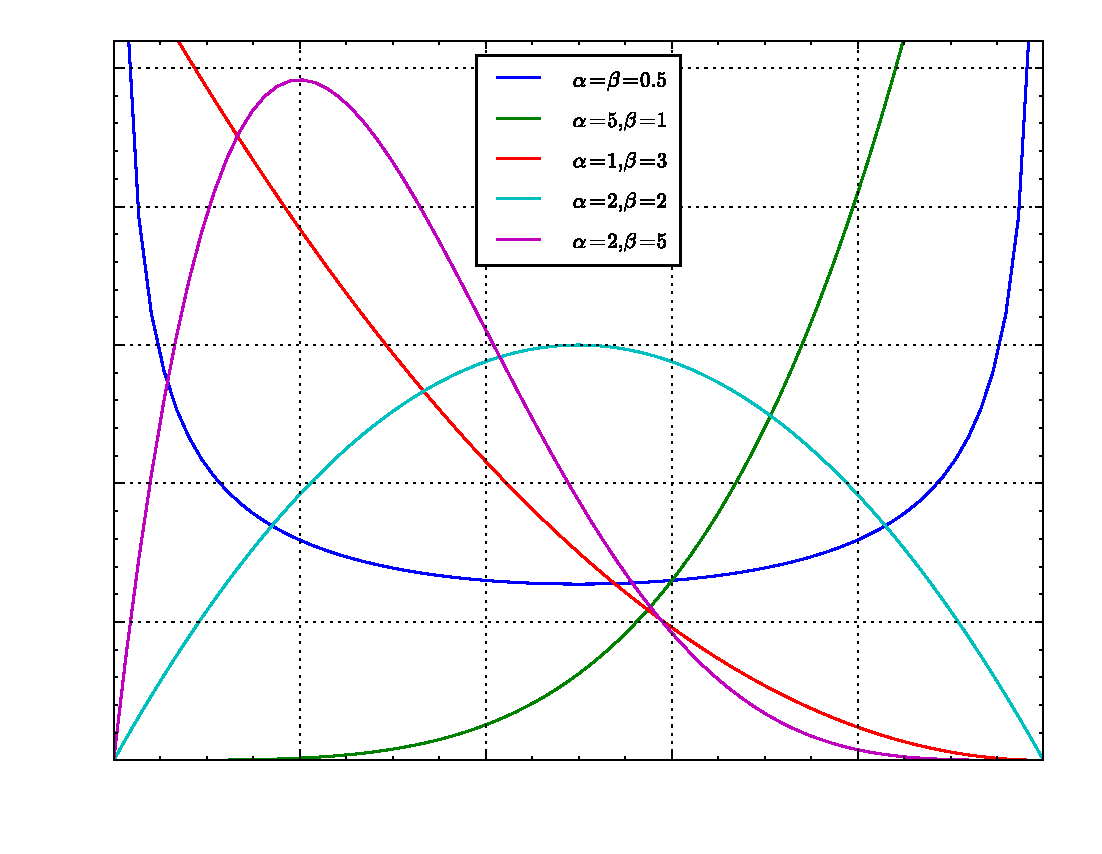
\includegraphics[width=0.8\textwidth]{figures/Beta_distribution_pdf.eps}
\caption[The beta distribution.]{The beta distribution for various shape parameters \citep{wiki_Beta}.  The distribution is non-zero on a finite range; it is this property that makes this distribution a candidate model for the neutron continuum.}
\label{fig:BetaGamma}
\end{figure}

This is an appropriate functional model because neutrons populating the continuum cannot have an energy greater than the ground-state neutron, and so its endpoint cannot extend past the center of the ground state neutron distribution; the beta distribution is non-zero only on a finite range.  The pulse-selected data set, however, does not constrain the tails of these functions well because the timing spectrum is not complete.  The non-pulse-selected data can help better constrain the fits in this region.

For the same bar, the non-pulse-selected spectrum should have the same features as the pulse-selected spectrum, but shifted and superimposed.  Fitting to the pulse-selected and non-pulse-selected histogram simultaneously greatly improves the fit because each bar of the neutron detector should measure the same beam-related spectrum for different runs, making it possible to model the non-pulse-selected spectrum as a shifted, scaled copy of the pulse-selected data.  The model used for the pulse-selected data is
% equation for pulse-selected spectrum
\begin{equation}
f_{PS} = B(x;\alpha,\beta) + Gaus_1 + Gaus_2 + Gaus_3 + DoubleGaus + Const_{PS}
\end{equation}
where $B(x;\alpha,\beta)$ is the Beta Distribution; $Gaus_1, Gaus_2, Gaus_3$ are Gaussian distributions describing prominent peaks in the continuum and the ground-state neutron peak; $DoubleGaus$ models the $\gamma$ peak.  These terms are needed to ensure a good overall fit and the contribution of each term is shown in {\fig}~\ref{fig:continuumModel}.  The non-pulse-selected data can be modeled by shifting the pulse-selected model by the interval between bunches $\tau$:
% equation for non-pulse-selected spectrum
\begin{equation}
R(f_{PS}(t) + f_{PS}(t+\tau) + f_{PS}(t+2\tau)) + Const_{NPS},
\label{eq:NPS_model}
\end{equation}
where $R$ is the ratio of total beam on target between the pulse-selected and non-pulse-selected runs.  Such a fit converges well and shows that the neutron continuum contributes less than 1\% to the extracted counts in the ground-state neutron peak.  

\begin{figure}[hp]
\centering
\subfloat[][]{
   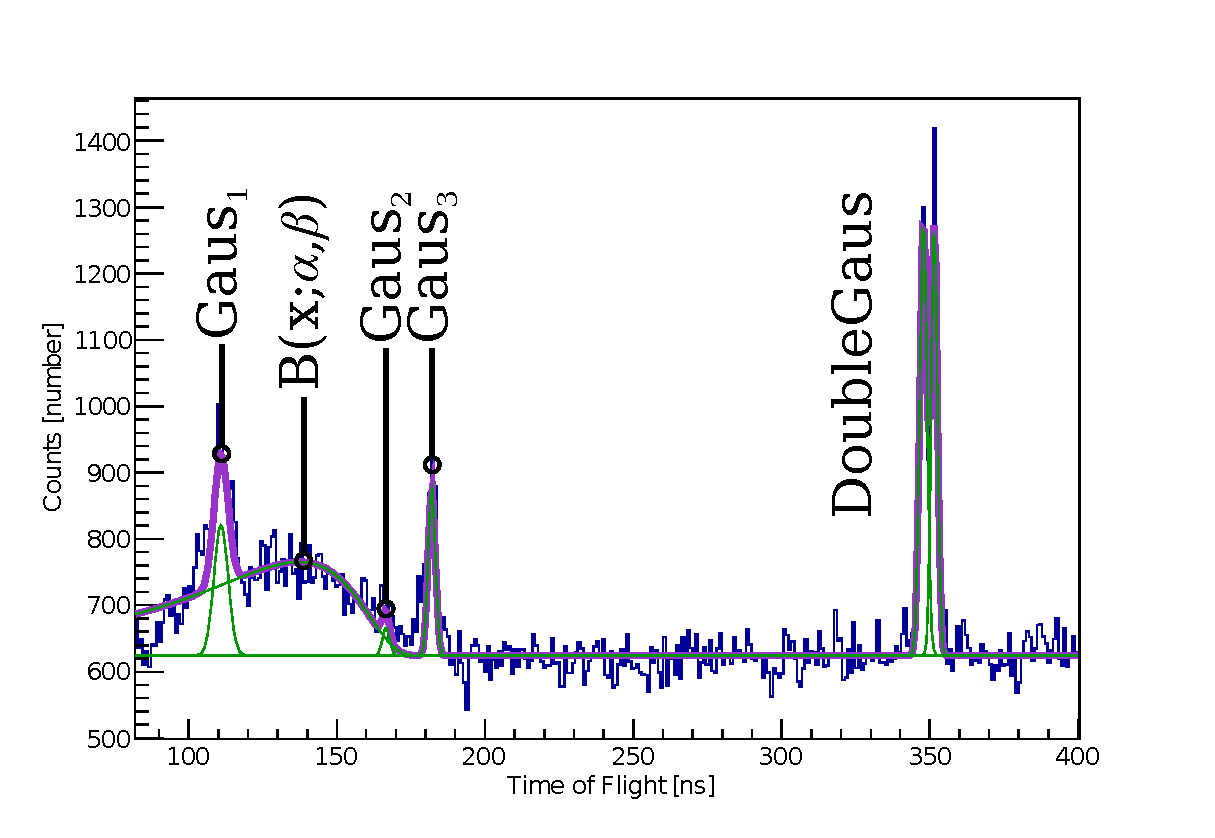
\includegraphics[width=0.6\textwidth]{figures/piecesOfFit0.eps}
}\\
\subfloat[][]{
   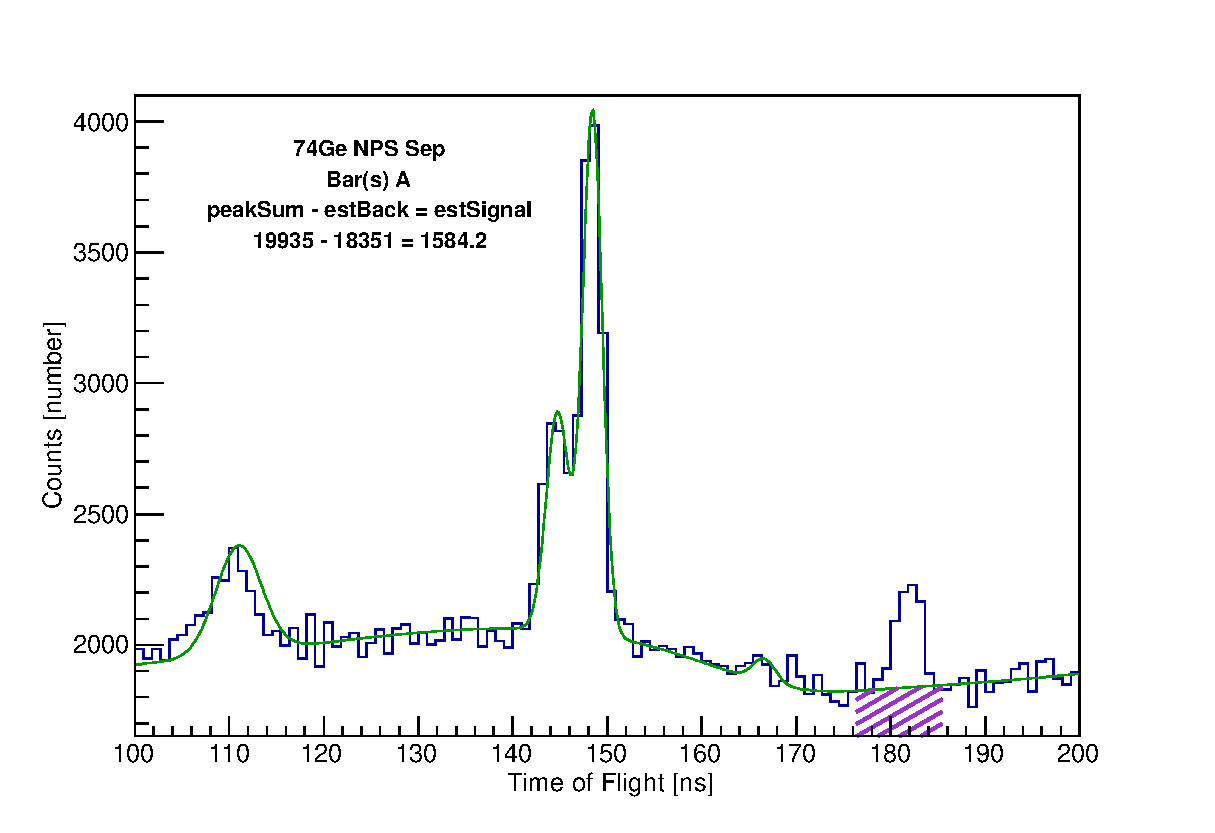
\includegraphics[width=0.6\textwidth]{figures/74Ge_NPS0.eps}
}
\caption[Functional fit to the pulse-selected timing spectrum.]{(a) The fit to the pulse-selected TOF spectrum of the forwardmost neutron detector bar (6.1$^{\circ}$).  The center and width of each gaussian is constrained for all bars simultaneously while the heights are fit for each bar independently.  (b) The timing spectrum of the non-pulse-selected beam is fit together with the pulse-selected spectrum.  The region of interest, the ground-state neutron peak, is highlighted but not used in the final data set because of its extreme sensitivity to the fit.}
\label{fig:continuumModel}
\end{figure}

The method used to extract the counts in the ground-state neutron peak is a direct summing of the counts from the peak region followed by subtraction of the estimated flat background from a linear fit.  The significant contributions to the estimated error is the statistical error of the sum of the peak region and the errorr associated with the low-energy cut.  Neither the fit to the flat background nor counts from the continuum contributed significant error to the extracted signal.  The systematic error contributions consist of the 10\% uncertainty in the efficiency and the 2\% uncertainty in target thickness.  The results are plotted in {\fig}~\ref{fig:PS_angularDistribution}.  See {\app}~\ref{app:crossSection} for a table of the values.

\begin{figure}[hp]
\centering
\subfloat[][]{
   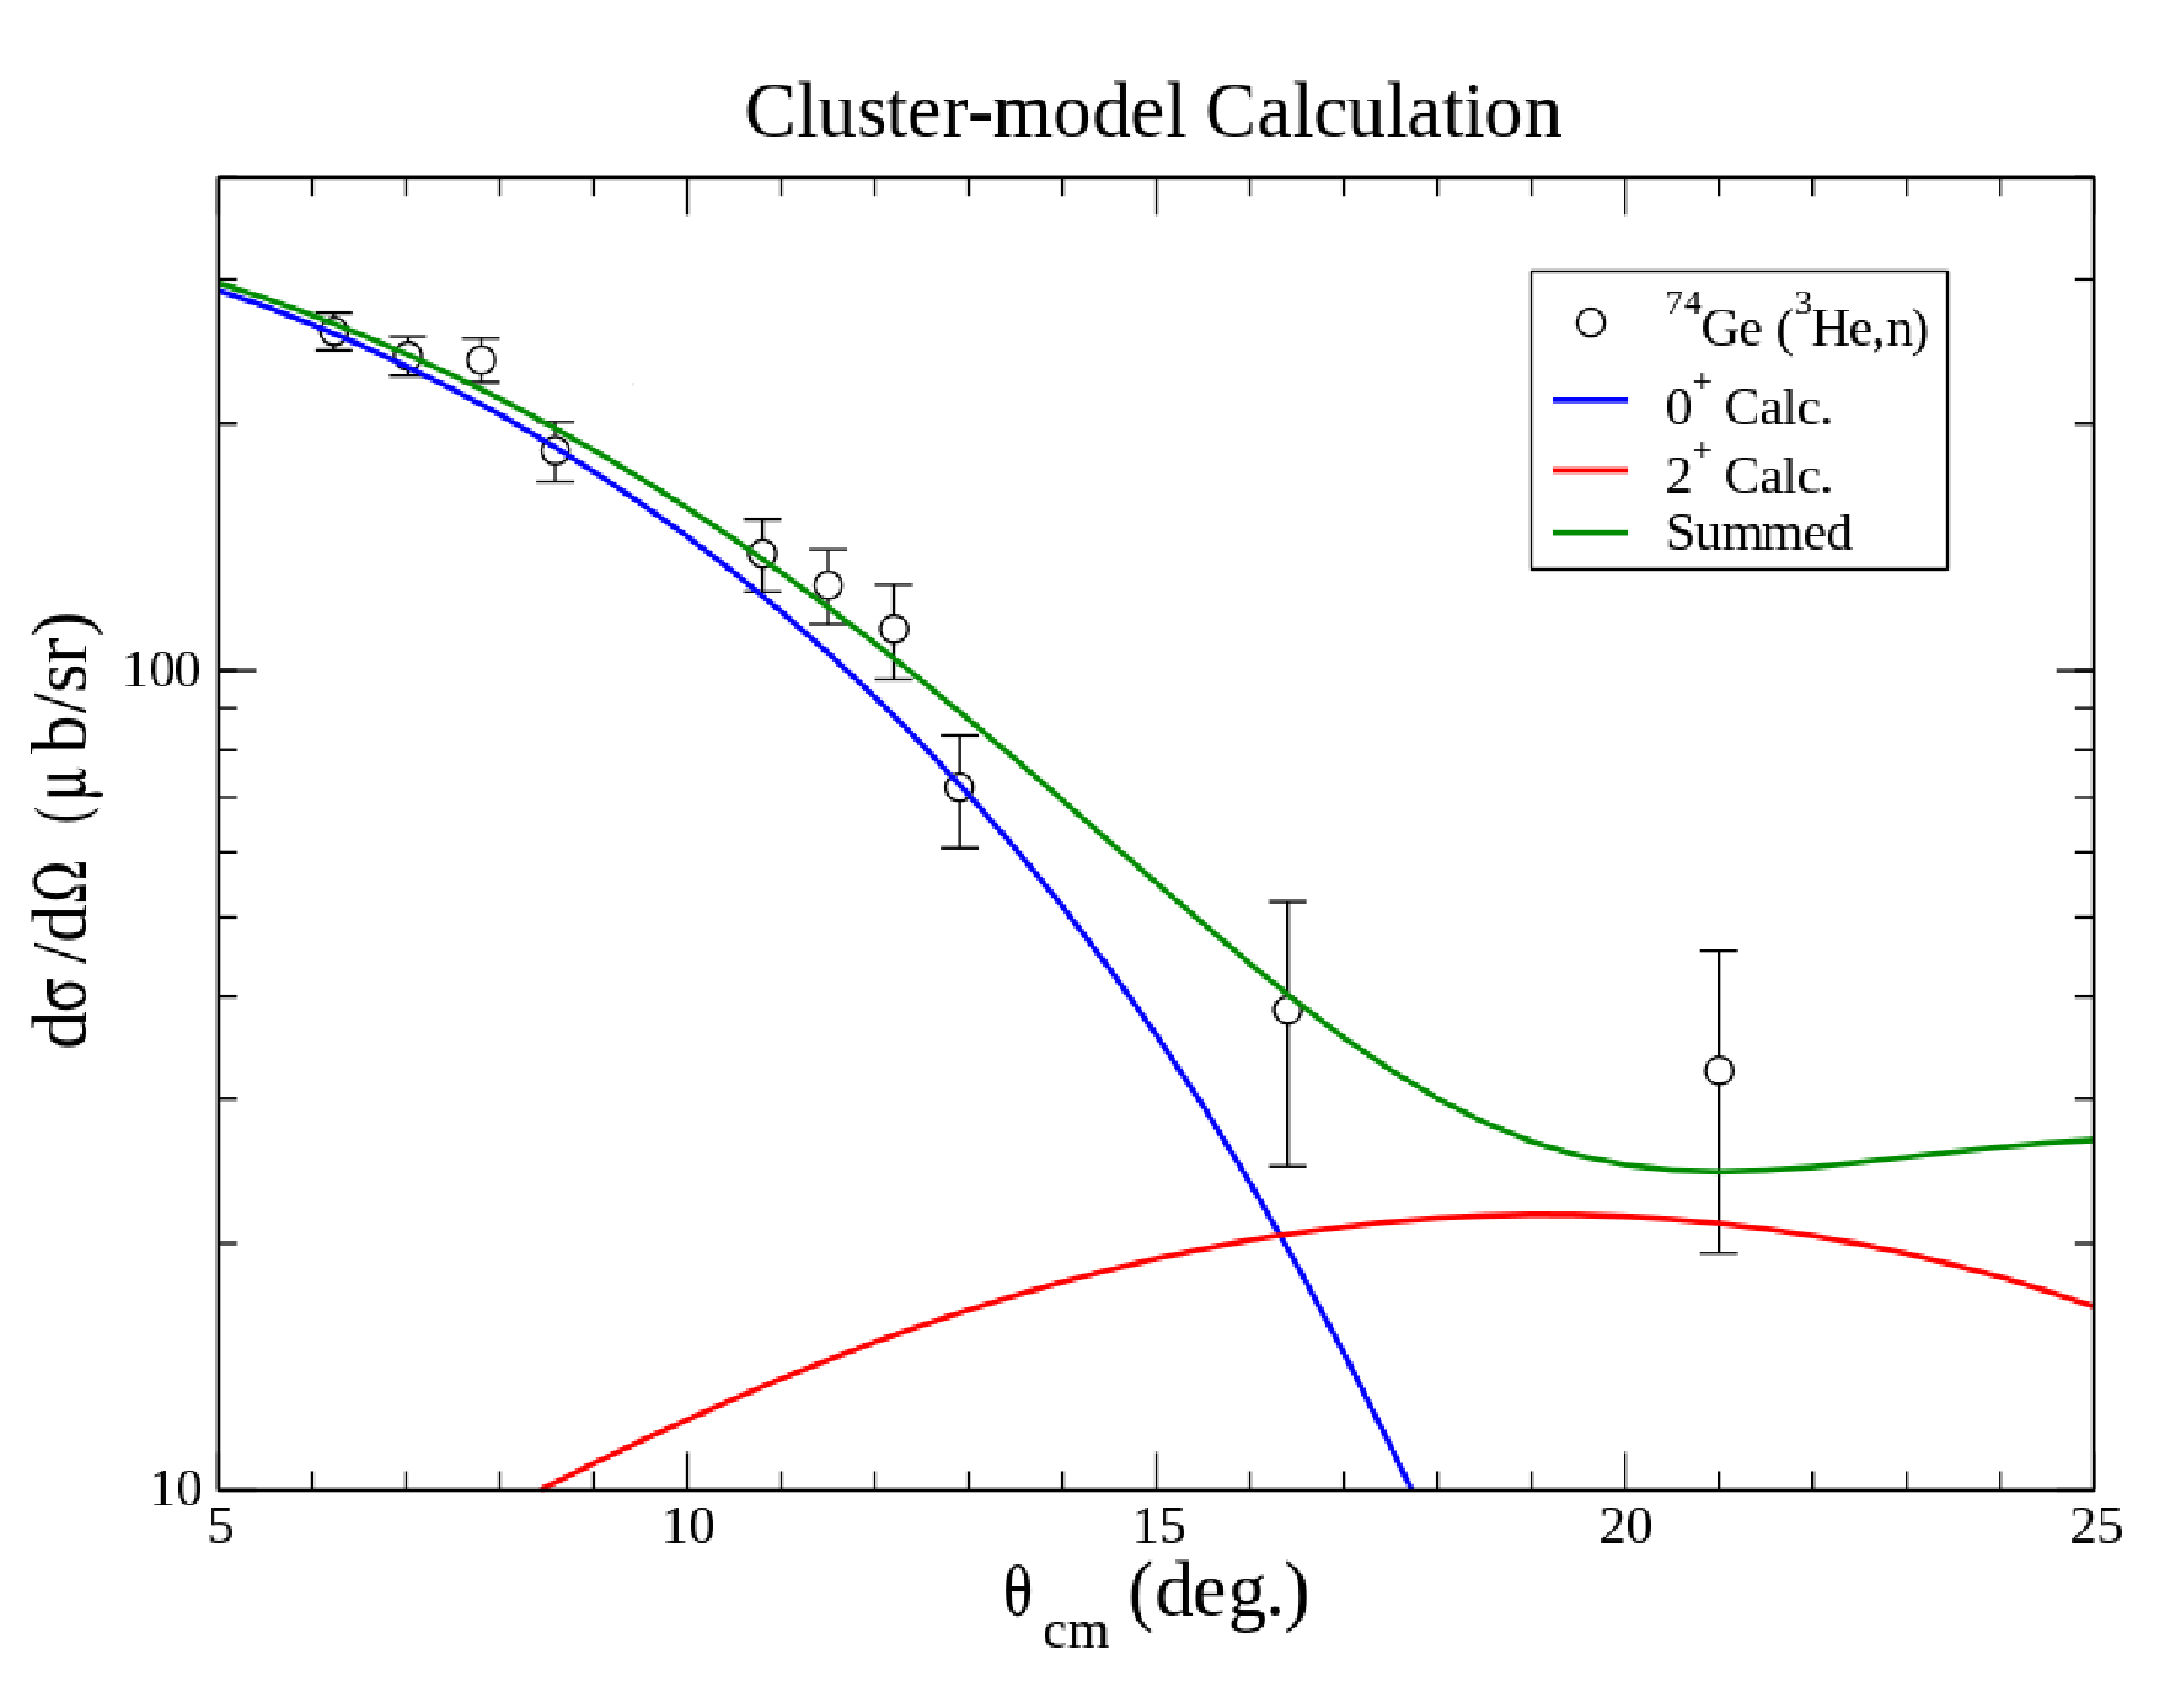
\includegraphics[width=0.5\textwidth]{figures/74Ge_angularDist.eps}
}
\subfloat[][]{
   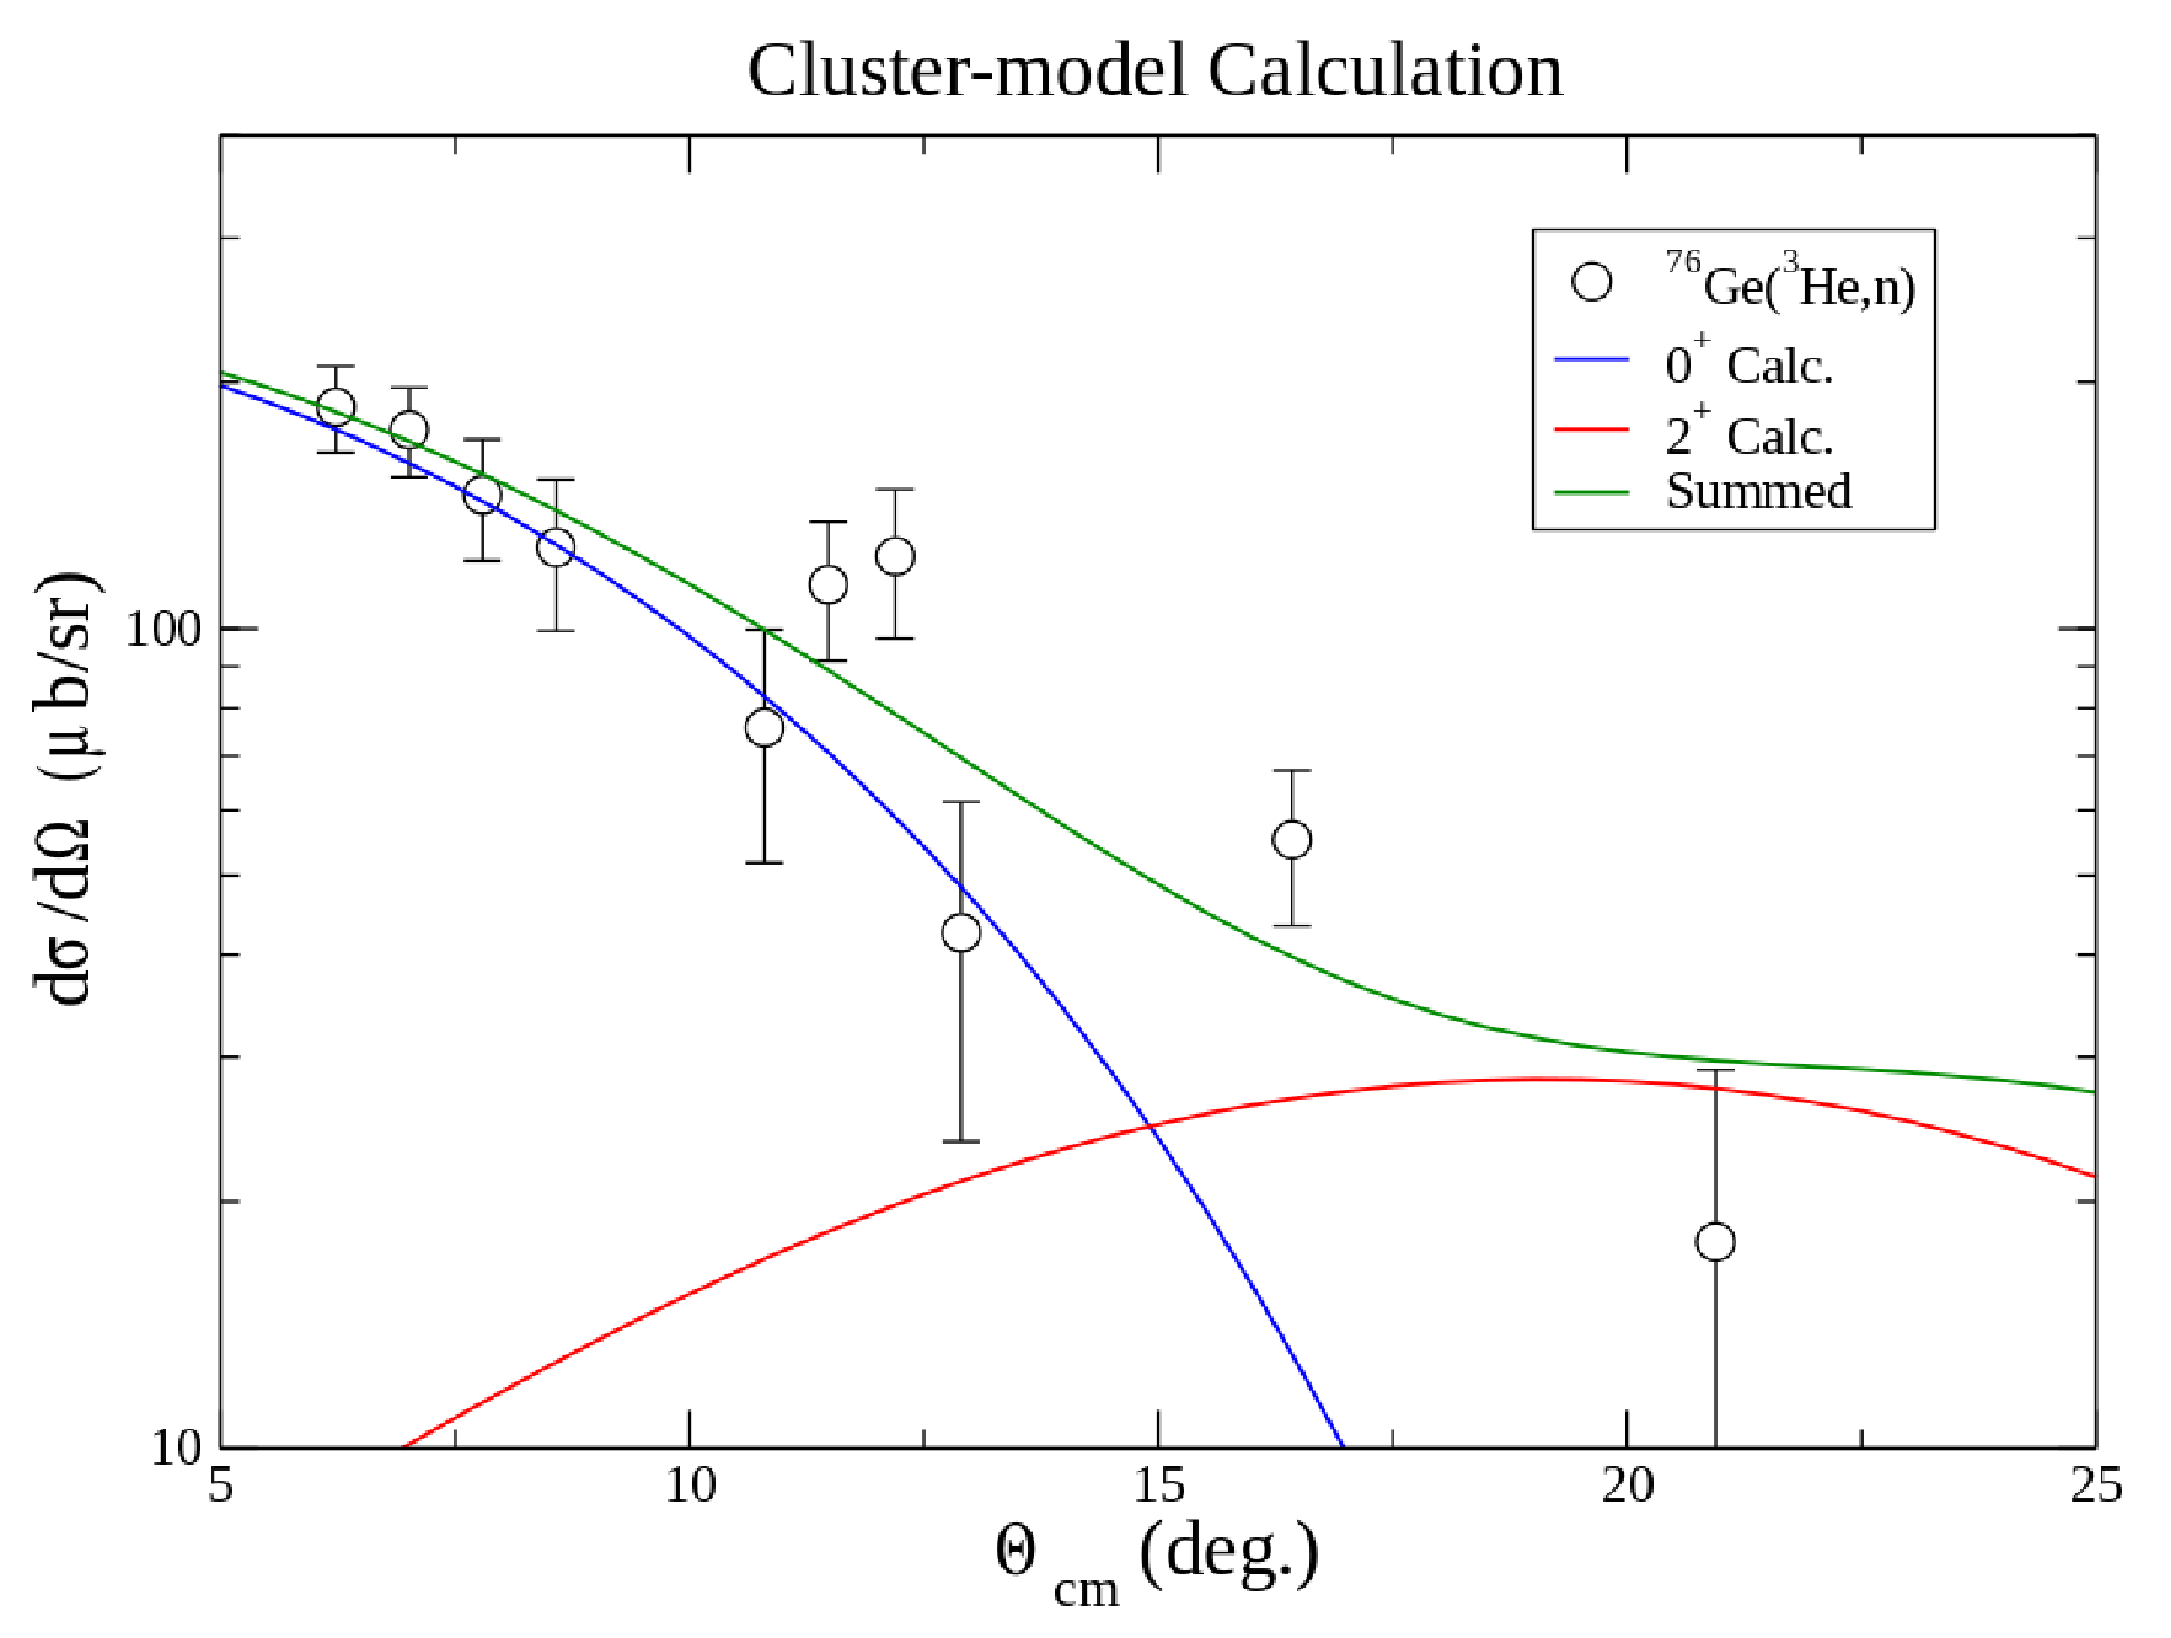
\includegraphics[width=0.5\textwidth]{figures/76Ge_angularDistribution.eps}
}
\caption[The angular distributions of the ground-state first excited state $^{74}$Ge($^3$He,n)$^{76}$Se and $^{76}$Ge($^3$He,n)$^{78}$Se.]{(a) The angular distributions of the ground-state first excited state $^{74}$Ge($^3$He,n)$^{76}$Se and (b) $^{76}$Ge($^3$He,n)$^{78}$Se.  In each graph, the two back-angle measurements are four-bar averages.  Because the timing resolution did not allow clear separation of the ground and first excited states, the integration window included both.  The DWBA fit to the data is described in {\sect}~\ref{sec:DWBA}.}
\label{fig:PS_angularDistribution}
\end{figure}
% edit figure so it JUST shows the data
\FloatBarrier

%A dedicated fitter may begin to wonder if there are as-yet-unused constraints that could provide an even more robust fit that would ensure a convergent fit for all angles.  One additional constraint concerns the ratio between the two datasets.  This ratio scales the amount of beam seen by one bar during the two data runs.  But each bar should see the same ratio!  Fitting all the bars simultaneously will provide a much-improved ratio.

\section{Placing a Limit on Excited \zp States}
\label{sec:zpLimit}
\begin{comment}
introduce 0+ peak and see when it becomes statistically significant
there will be different limits for different energies!  because of the evaporation background
\end{comment}
A primary aim of this experiment is to investigate the distribution of \zp strength, making it important to either measure or place a limit on the cross sections of excited \zp states.  Because the non-pulse-selected data have significant, complicated background, only the pulse-selected data sets were used for this analysis.  Because the \zp cross section is largest at forward angles, spectra from the three forwardmost detectors was summed to make the TOF spectrum used in this analysis.  These three detectors span lab angles 6.1$^{\circ}$ to 7.7$^{\circ}$.  The fourth detector, at 8.4$^{\circ}$, was not included because the \zp cross sections noticeably decline at this angle.  Including this detector or any detectors beyond it would have introduced background without contributing significant signal, worsening the sensitivity.    

% expand on states that were observed?
No obvious \zp states were observed above the neutron continuum for \Ge{74} or \Ge{76} targets.  A limit on the cross section of \zp states as a function of energy can be determined by solving for the number of counts $S$ necessary to be consistent with zero within $i$ standard deviations $\sigma_S$:
\begin{equation}
S = P - B = i\sigma_S,
\end{equation}
where $P$ is the number of counts in the potential signal region and $B$ is an estimate of the counts in that same region.  In this case, sideband subtraction is the most appropriate method of determining $B$ because the shape of the continuum is not well-known and attempting to fit it functionally could introduce additional systematic error.  The error associated with the signal-induced counts $S$ is then
\begin{equation}
\sigma_S = i\sqrt{P+B} \approx i\sqrt{S+B+B} = i\sqrt{S+2B}.
\end{equation}
The number of signal counts $S$ can now be written as a function of the background counts $B$ and the desired level of certainty, $i$:
\begin{equation}
S = \frac{i^2 \pm \sqrt{i^4 + 8i^2B}}{2}.
\end{equation}
Note that the number of background counts $B$ scales with the chosen integration window.  The limits shown were calculated with an integration window of $\sim$7~ns, wide enough to include 95\% of the peak.  This width was held constant across the region tested for excited \zp states, which was appropriate because the width of the timing peak at this energy is dominated by the spread in beam bunching, target effects, and detector timing resolution, none of which change for neutrons within 2~MeV of the ground state neutrons.

The $2\sigma$ limit on the cross section for excited \zp states in \Ge{74} and \Ge{76} is shown in {\fig}~\ref{fig:differentLimits}.  The $2\sigma$ limit was chosen in order to have 95\% confidence in the existence of a peak.  A simulation of peaks at the 2$\sigma_S$ limit is shown in {\fig}~\ref{fig:differentLimits}.  It is important to note that the Q-value dependence of the cross section has a significant impact on the limit.  As the excitation energy of the product nucleus increases, the Q-value decreases and the cross section increases.  This relationship for \reaction is calculated with DWBA and is shown in {\fig}~\ref{fig:QvalDependence}.

The Q-value dependence must be factored out of the count limit obtained directly from the TOF histogram.  In general, this is advantageous, as searching for higher excited \zp states implies a lower Q value and therefore greater sensitivity.  However, at very high excitation energies, the decreasing detector efficiency takes over and the limit begins trending upwards.

\begin{figure}[hp]
\centering
\includegraphics[width=0.8\textwidth]{figures/SigmaVsQ.eps}
\caption[The Q-value dependence of the zero-degree cross section of $^{74}$Ge(\He{3},n) and $^{76}$Ge(\He{3},n).]{The Q-value dependence of the zero-degree cross section of $^{74}$Ge(\He{3},n) and $^{76}$Ge(\He{3},n).  The \He{3} is incident at 16~MeV.  Solid lines indicate the dependence on the Q-value only, while the dashed lines show the dependence moderated by the detector efficiency.  Symbols indicate known \zp states.}
\label{fig:QvalDependence}
\end{figure}

\begin{figure}[hp]
\centering
\subfloat[][]{
   \includegraphics[height=0.4\textheight]{figures/DetLimits.eps}
} \\
\subfloat[][]{
   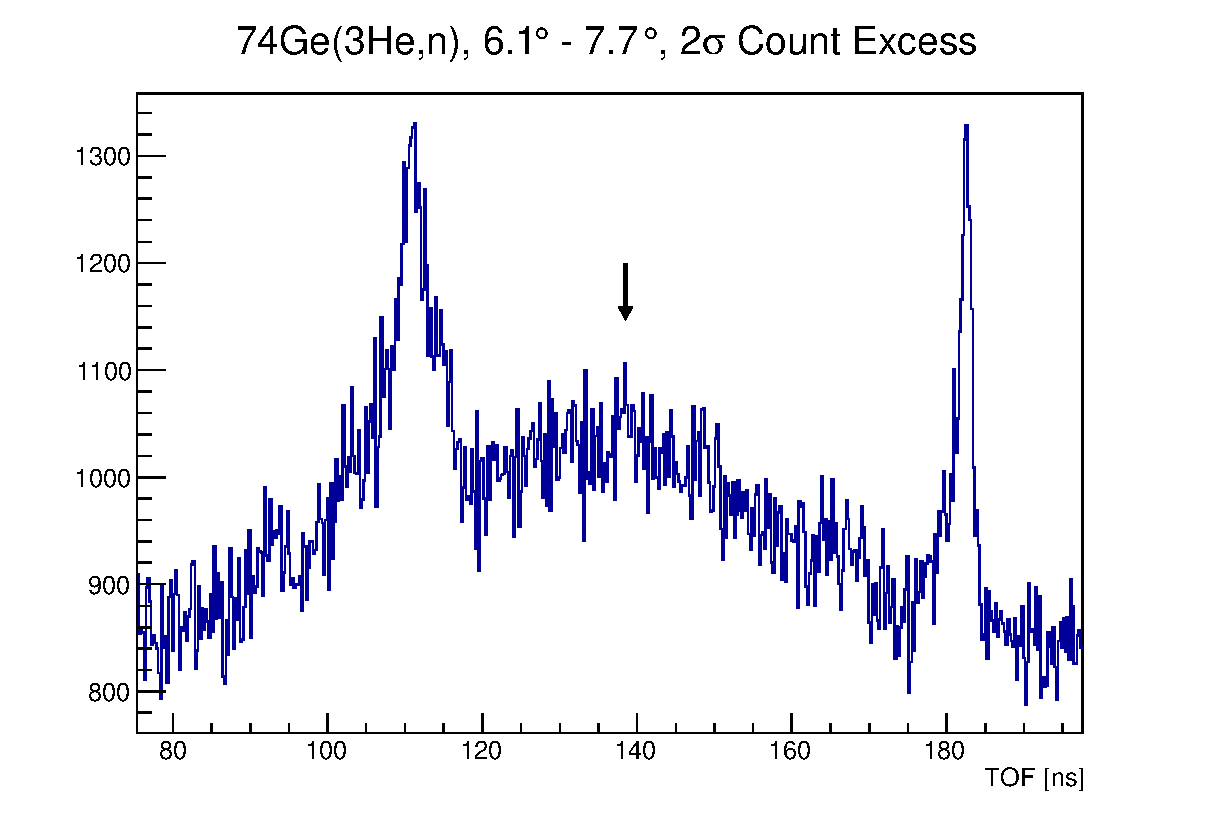
\includegraphics[height=0.2\textheight]{figures/74Ge_2sigma_limit.eps}
}
\hspace{8pt}
\subfloat[][]{
   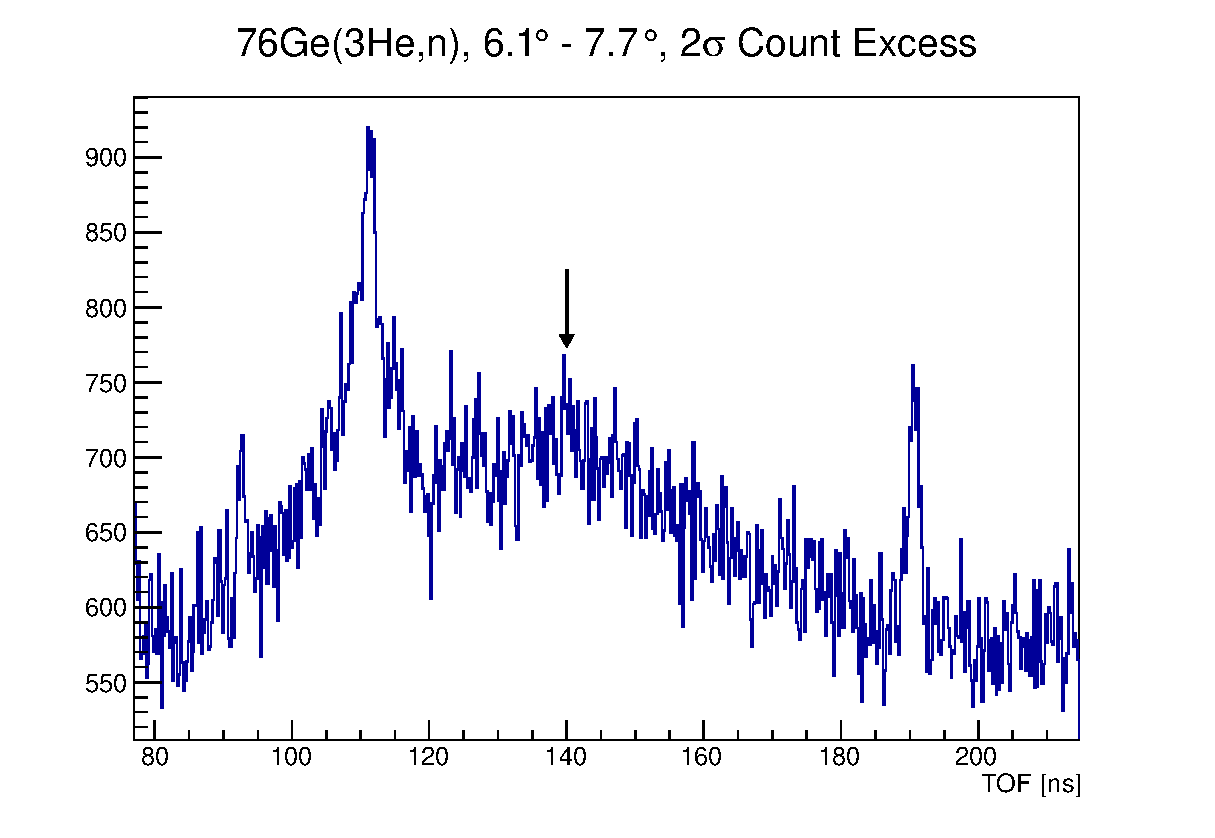
\includegraphics[height=0.2\textheight]{figures/76Ge_2sigma_limit.eps}
}
\caption[Limit on excited \zp states as a percentage of the ground-state cross section for $^{74}$Ge and $^{76}$Ge.]{(a) Limit on excited \zp states as a percentage of the ground-state cross section for $^{74}$Ge (lower, in red) and $^{76}$Ge (above, in blue).  It is assumed that the width of any states in this region will be the same as the width of the ground-state peak.  The limit is unreliable for neutrons arriving at times less than 120~ns relative to the $\gamma$ peak because of the broad neutron peak due to oxygen contamination in the targets as can be seen in (b).  The detection limit is therefore cut off at that point.  (b) The effect of a signal with 2$\sigma$ significance is simulated for $^{74}$Ge.  (c) The effect of a signal with 2$\sigma$ significance is simulated for  $^{76}$Ge.}
\label{fig:differentLimits}
\end{figure}
% excitation energy, not timing
% don't show past big peak
\FloatBarrier

\section{Fitting the \zp Ground State}
\label{sec:DWBA}
\begin{comment}
DWBA calculation
shell model
f$^2$, p$^2$ state strength ("form factor")
\end{comment}
The ground-state cross section of $^{74}$Ge($^3$He,n) is larger than that of $^{76}$Ge($^3$He,n).  One may wonder if the lower $^{76}$Ge($^3$He,n) cross section is due to missing \zp strength or is instead an expected result of, for example, the different kinematics of the reaction.  One way to check is to calculate the zero-degree cross section with a model that assumes the \zp strength to be in the ground state and compare this to the measured values.  The zero-degree ground-state cross section can be determined by fitting the experimentally-determined angular distribution of the ground and first excited state together with DWBA and extrapolating the result to zero degrees.  The code Fresco \citep{Fresco}, used to perform the DWBA calculations, requires the binding potential for the di-proton in the \He{3} and \Ge{74} nuclei as well as the optical-model potentials experienced by the incoming \He{3} nucleus and the outgoing neutron.  Typical values for the parameters of these potentials are given in {\tab}~\ref{tab:typicalPotentials}, where the optical-model potentials used for the \He{3} and neutron are Becchetti-Greenlees \citep{Becchetti_3HePotential} and Koning-Delaroche \citep{Koning_neutronPotential}, respectively.  The results of the fit to the measured angular distributions are shown in {\fig}~\ref{fig:PS_angularDistribution}.
\begin{sidewaystable}\footnotesize
\ra{1.1}
\caption[\uppercase{potential parameters for DWBA analysis}]{\\\label{tab:typicalPotentials} \uppercase{potential parameters for DWBA analysis}}
%\begin{ruledtabular}
\begin{tabular}{ccccccccccccccccc}\toprule
Particle & V$_0$ & r$_{\text{R}}$ & a$_{\text{R}}$ & V$_{\text{SO}}$ & r$_{\text{SO}}$ & a$_{\text{SO}}$ & W & r$_{\text{W}}$ & a$_{\text{W}}$ & W$_{\text{D}}$ & r$_{\text{WD}}$ & a$_{\text{WD}}$ & W$_{\text{SO}}$ & r$_{\text{WSO}}$ & a$_{\text{WSO}}$ & r$_{\text{c}}$ \\
\midrule
$^{3}$He (BG) & 157.1 & 1.20 & 0.72 & 2.50 & 1.20 & 0.72 & 43.4 & 1.40 & 0.88 & - & - & - & - & - & - & 1.30\\
$^{3}$He (U) & 175.4 & 1.14 & 0.71 & - & - & - & 19.9 & 1.53 & 0.85 & 9.13(N-Z)/A & 1.53 & 1.85 & - & - & - & 1.4\\
$^{3}$He (GDP08) & 118.92 & 4.98 & 0.82 & 1.38 & 3.87 & 0.13 & 1.71 & 5.37 & 0.84 & 23.09 & 5.37 & 0.84 & - & - & - & 5.33\\

n (BG) & 45.27 & 1.21 & 0.54 & 5.57 & 1.03 & 0.59 & 1.18 & 1.21 & 0.54 & 6.76 & 1.34 & 0.53 & -0.07 & 1.03 & 0.59 & -\\
n (KD) & 45.47 & 1.21 & 0.67 & 5.55 & 1.03 & 0.59 & 1.24 & 1.21 & 0.67 & 6.6 & 1.28 & 0.53 & -0.076 & 1.03 & 0.59 & -\\

$^3$He bound state & 76.6$^{\mathbf{\dagger}}$ & 1.175 & 0.65 & - & - & - & - & - & - & - & - & - & - & - & - & 1.30\\

Se bound state & 100$^{\mathbf{\dagger}}$ & 1.30 & 0.65 & - & - & - & - & - & - & - & - & - & - & - & - & 1.30\\
\bottomrule
% combine with other table of potential parameters
\end{tabular}
%\end{ruledtabular}
\begin{flushleft}
{\footnotesize NOTE:
Optical and bound-state potentials used in the DWBA analysis, see the text for details of the calculations. Both optical-model potentials vary slowly with $N$, $Z$ and $E$; the values given here are typical. $^{\mathbf{\dagger}}$Starting value; adjusted to reproduce the experimentally measured binding energy.}
\end{flushleft}
\end{sidewaystable}
% and now the figure
\begin{figure}[!htbp]
\centering
\subfloat[][]{
   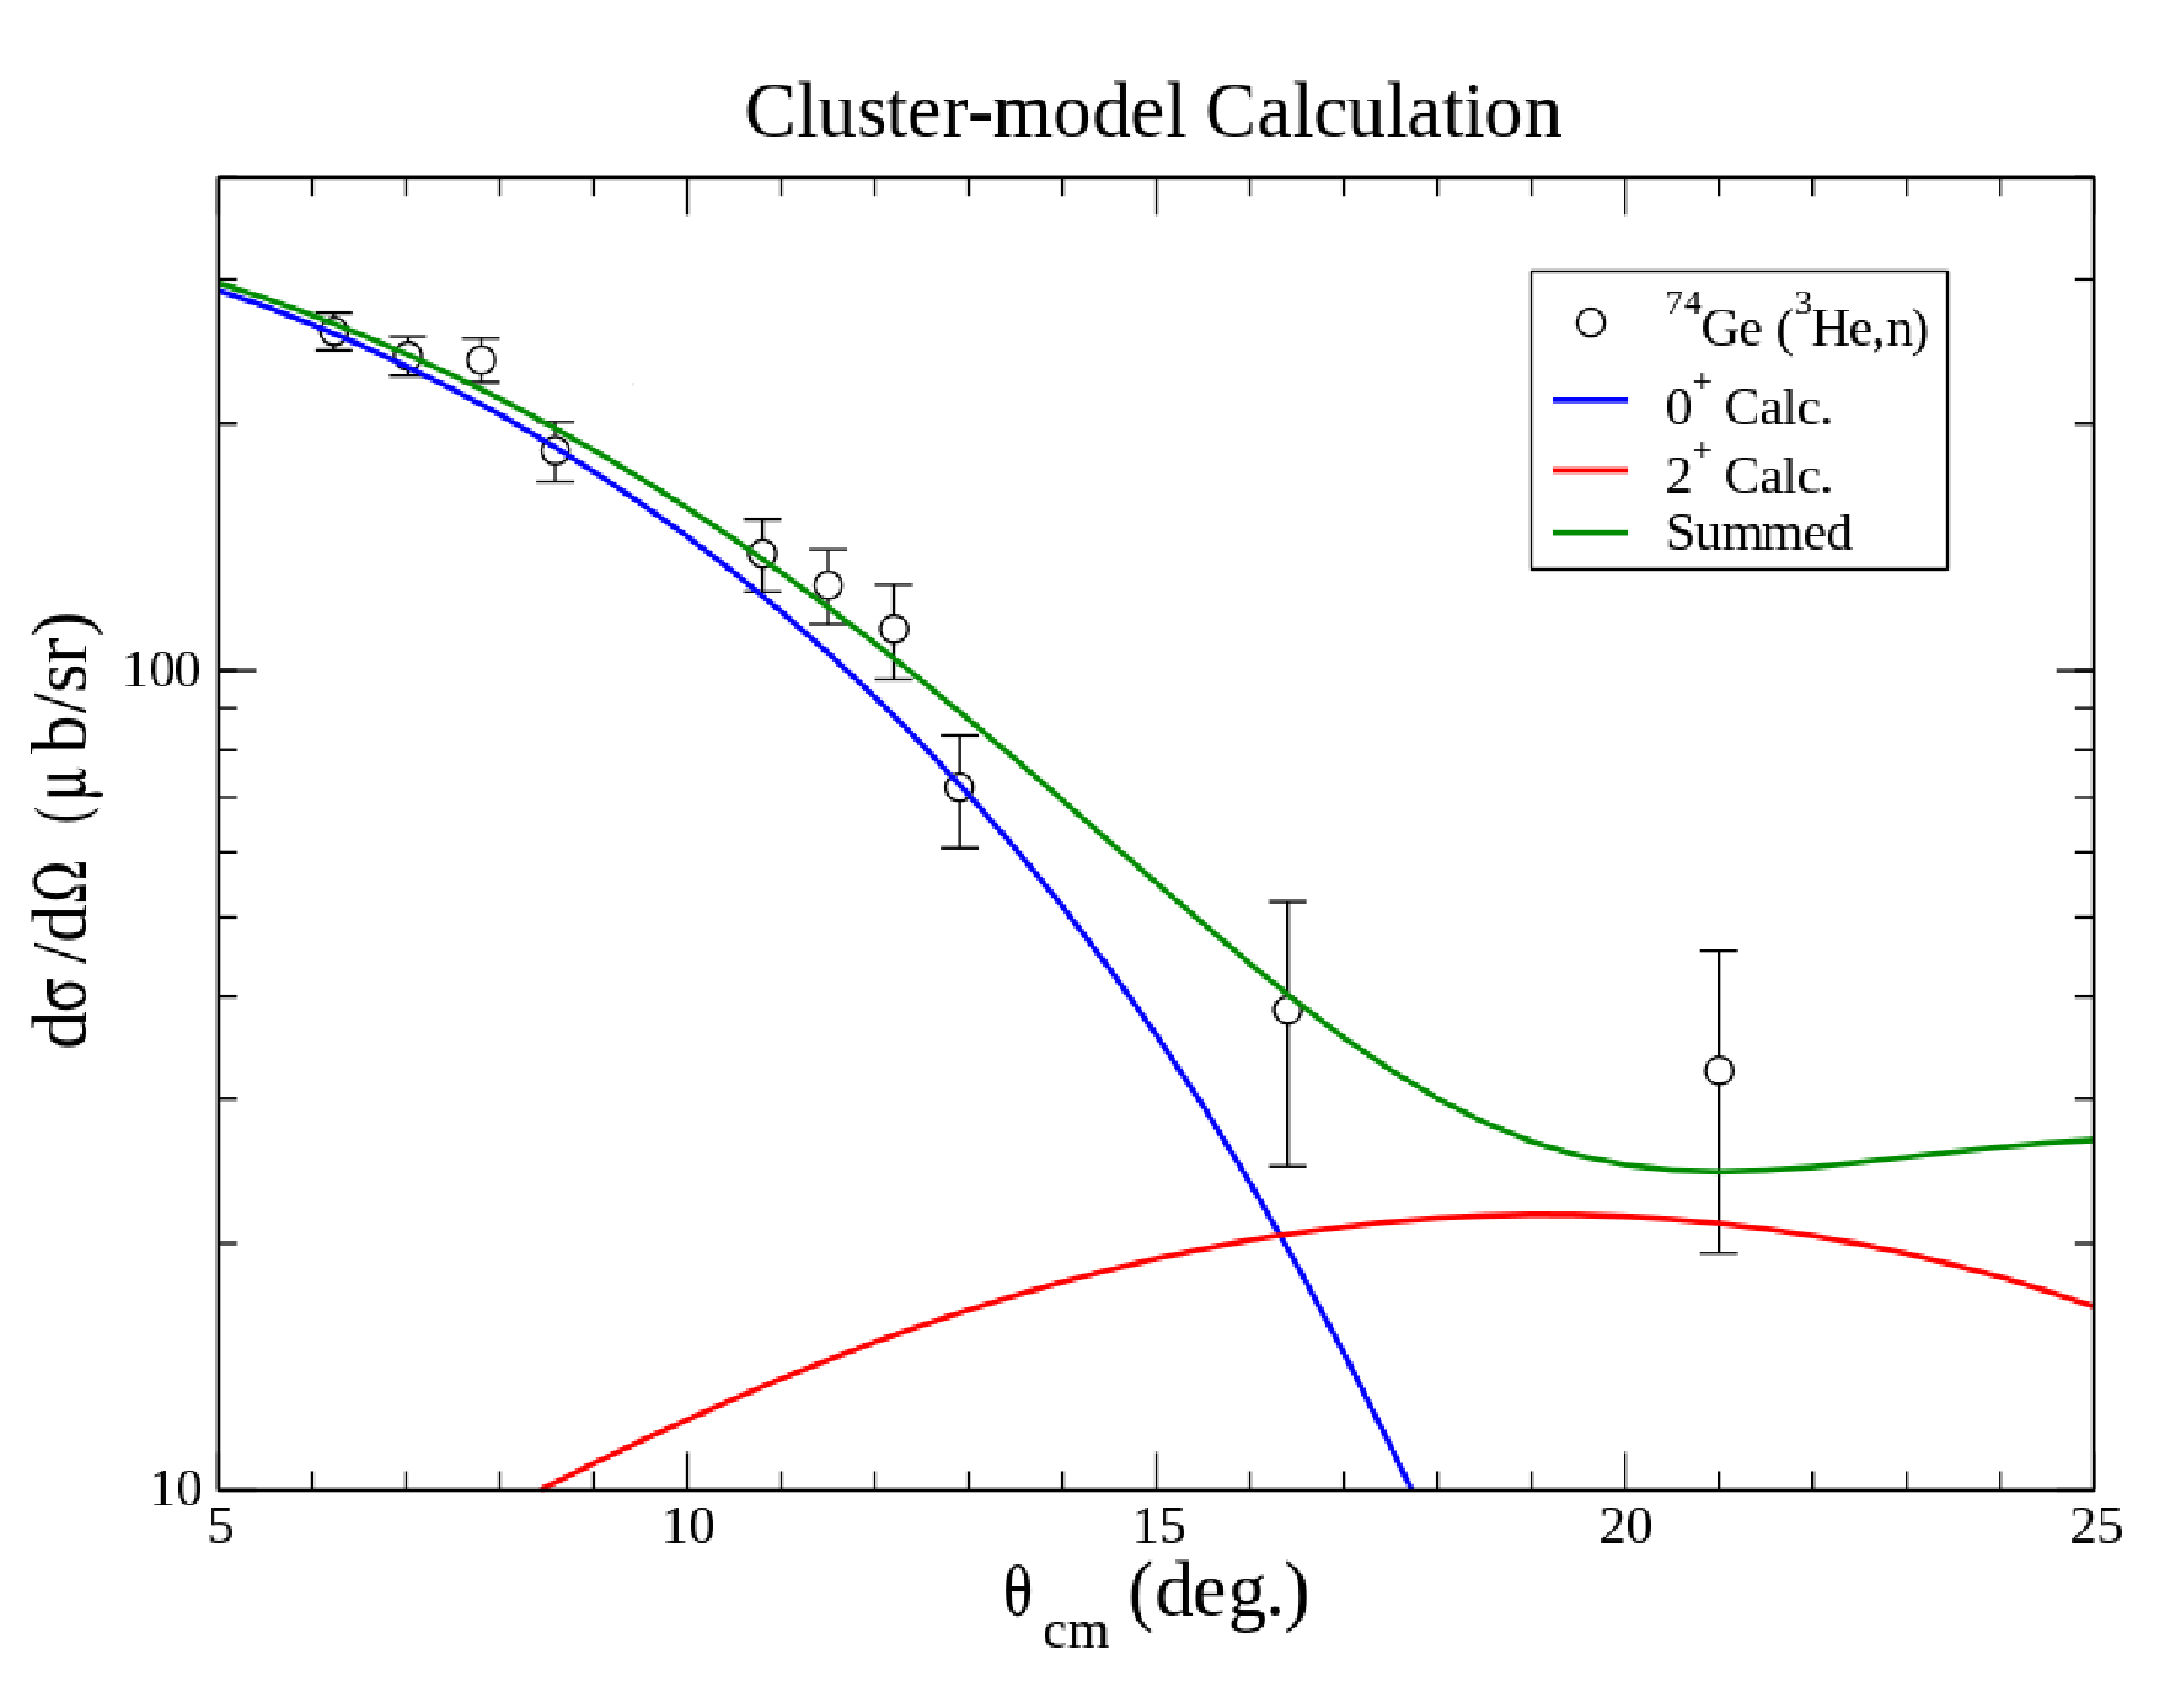
\includegraphics[width=1.0\textwidth]{figures/74Ge_angularDist.eps}
}\\
\subfloat[][]{
   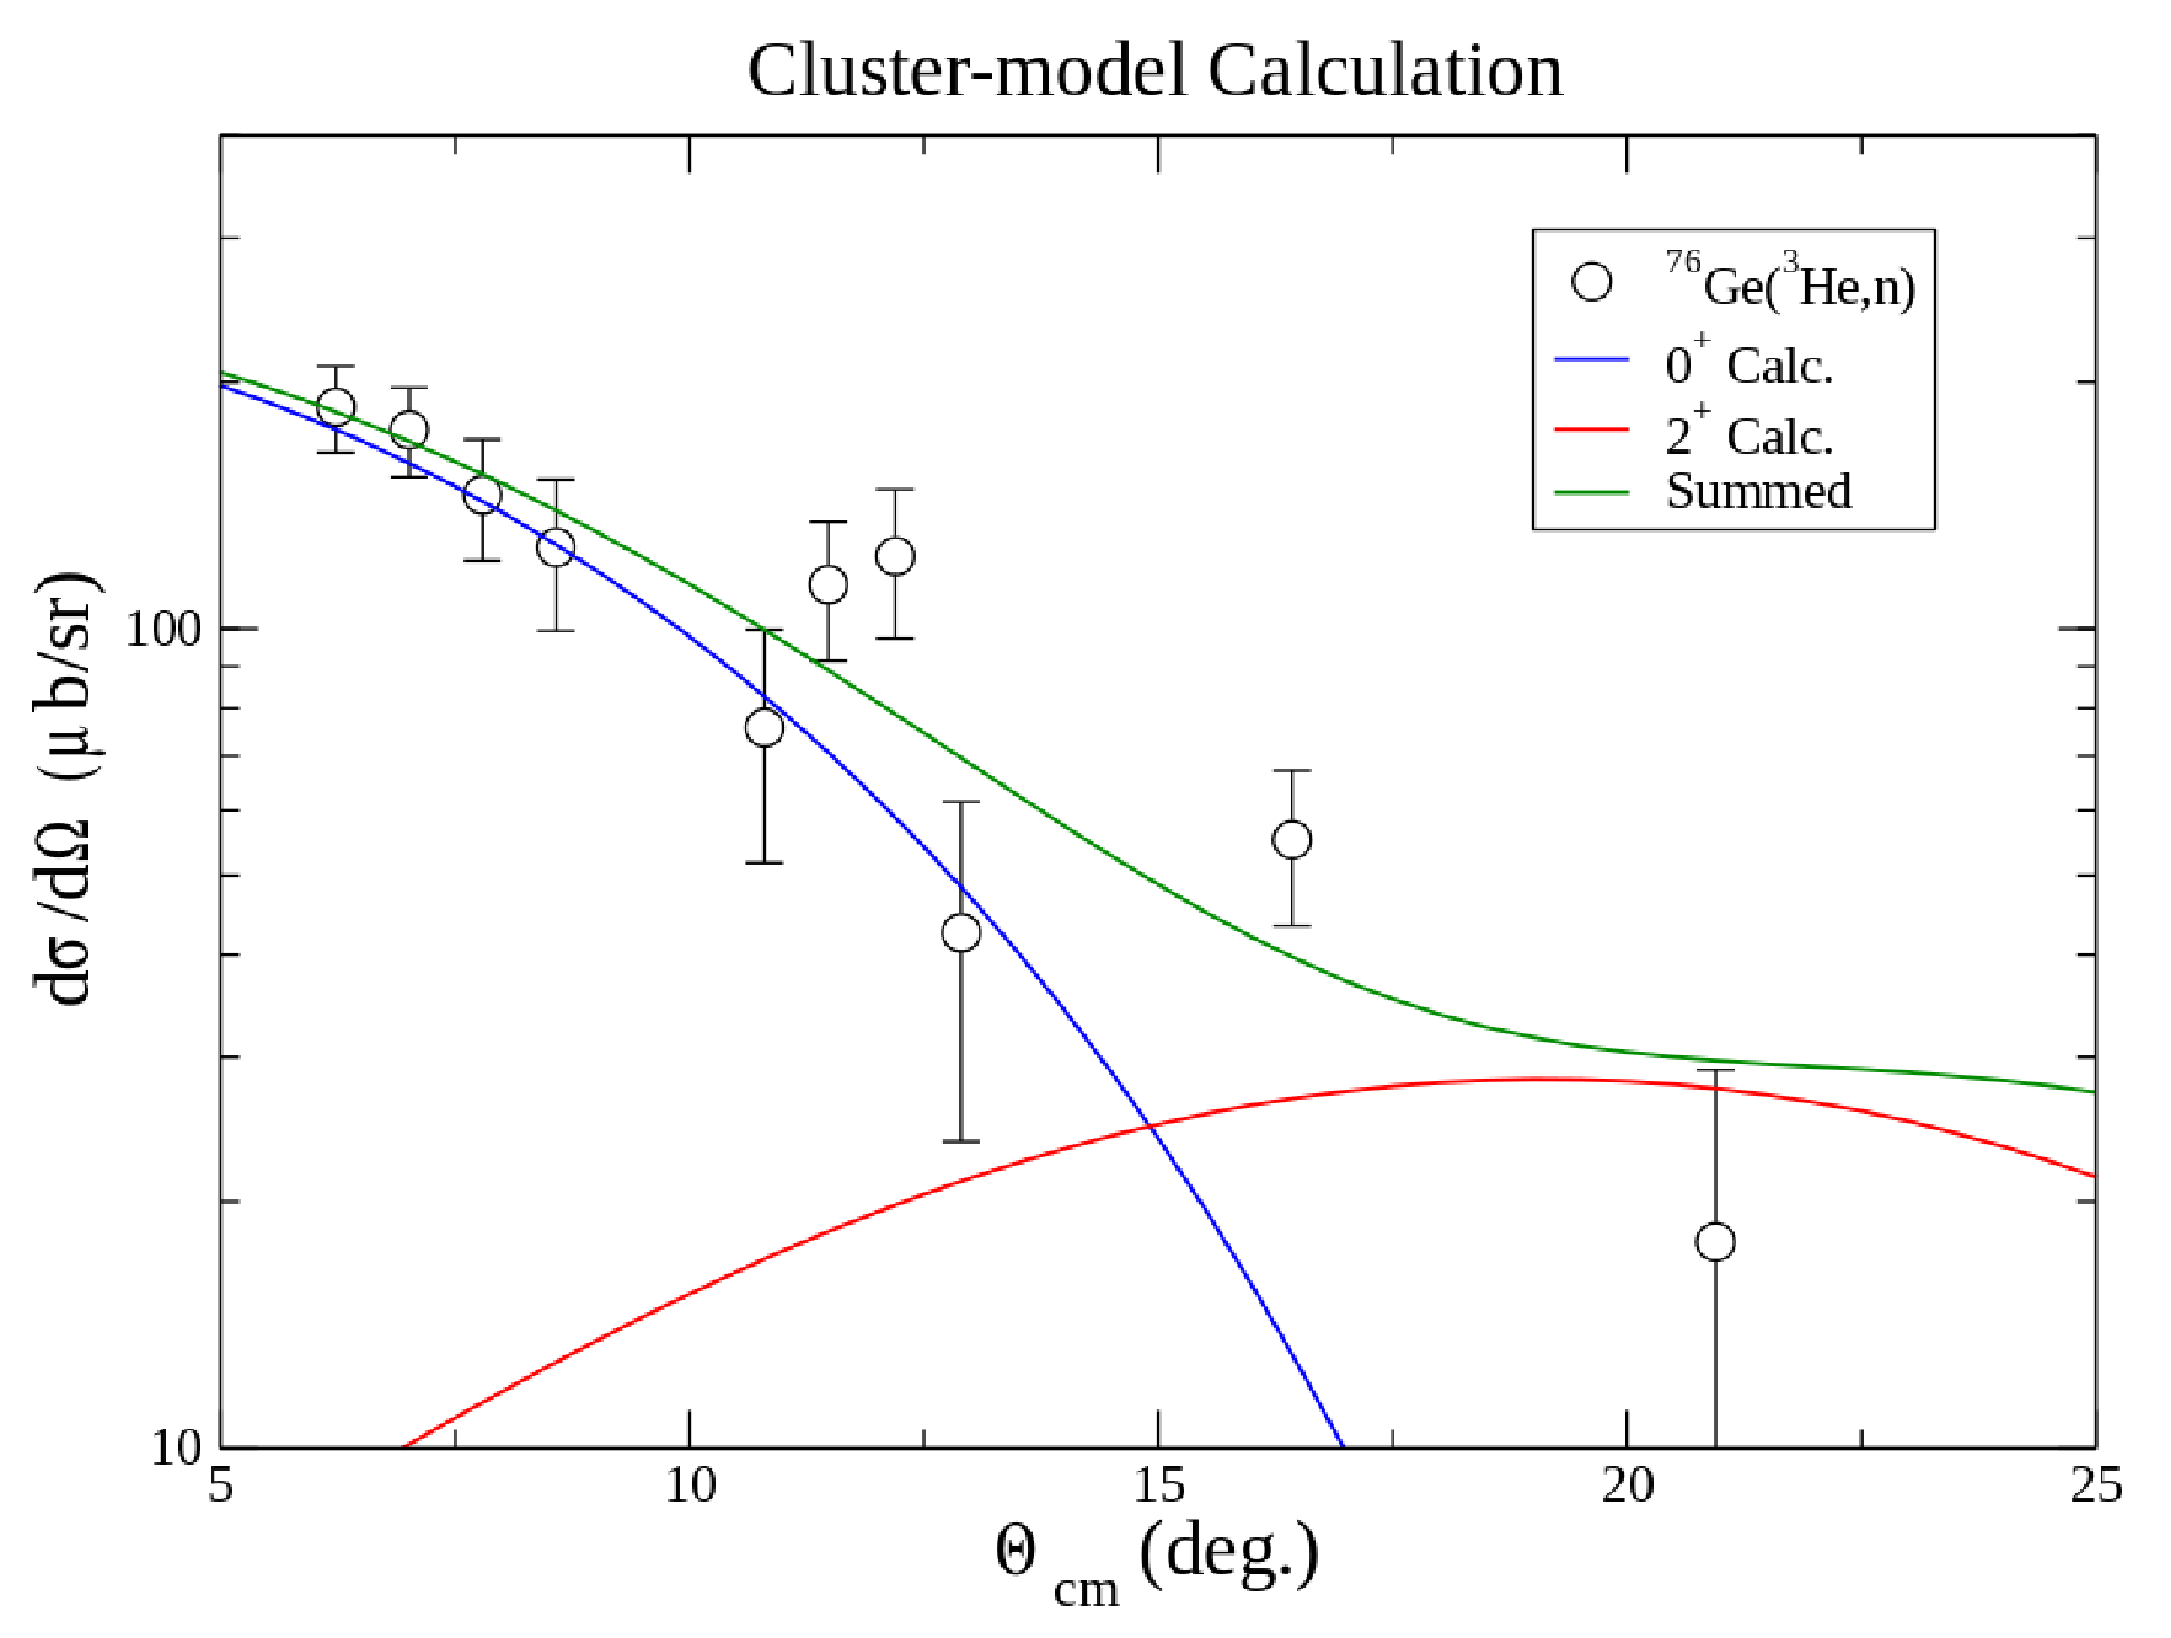
\includegraphics[width=1.0\textwidth]{figures/76Ge_angularDistribution.eps}
}
\caption[The angular distributions of $^{74}$Ge($^3$He,n)$^{76}$Se and $^{76}$Ge($^3$He,n)$^{78}$Se.]{(a) The angular distributions of $^{74}$Ge($^3$He,n)$^{76}$Se and (b) $^{76}$Ge($^3$He,n)$^{78}$Se.  In each graph, the two back-angle measurements are four-bar averages.  Because the timing resolution did not allow clear separation of the ground and first excited states, the integration window included both.  The sum of the DWBA calculations for the ground and first-excited states has a $\chi^2$ of 0.7 for the \Ge{74} data and 1.3 for the \Ge{76} data.}
\label{fig:PS_angularDistribution}
\end{figure}
 
The cluster model is sensitive to the parameters used to describe the potentials of the interacting nuclei.  The sensitivity of the extracted zero-degree cross section on the bound-state radius parameter, the neutron optical-model potential, and the principal quantum number were all investigated.  While changing the bound-state radius strongly affects the normalization, it does not appreciably affect the shape of the angular distribution between 0$^{\circ}$ and 20$^{\circ}$ and therefore does not impact the ratio of ground-state to first-excited-state cross section at zero degrees.  Using the Becchetti-Greenlees neutron potential rather than the Koning-Delaroche potential does not strongly affect the angular distribution, nor does changing the principal quantum number.  The effect of varying these parameters is shown in {\fig}~\ref{fig:varyParam}.  The dependence of the cross section for various \He{3} optical-model potentials was also explored and found to result in little difference in the trend in the zero-degree cross sections of \Ge{74} and \Ge{76}.  See {\tab}~\ref{tab:typicalPotentials} for the tested parameter ranges and {\fig}~\ref{fig:parameterSensitivity} for their impact on the relative cross section.

As discussed in {\chap}~\ref{chap:nucl}, both the cluster and Bayman-Kallio models typically describe the same shape for the $L=0$ angular distribution, but neither model typically reproduces the absolute cross section.  In the case of the $^{58,60,62,64}$Ni and $^{88}$Sr isotopes, however, the cluster model reproduces the trend as a function of the neutron number rather well.  This agreement is shown in {\fig}~\ref{fig:nickelTrend}, where all cross sections have been normalized to $^{74}$Ge.  The cluster model, then, accurately describes the trend when adding protons to \fpg shell nuclei in this mass region.  Cluster model calculations of the $^{74}$Ge($^3$He,n)$^{76}$Se and $^{76}$Ge($^3$He,n)$^{78}$Se reactions show that the smaller cross section of the $^{76}$Ge($^3$He,n)$^{78}$Se reaction is due to the Q-value dependence reproduced by DWBA and not to ground-state loss of \zp strength.   The cross sections measured for \reaction are consistent with DWBA predictions and the data suggest that the $l=0$ pair-transfer strength to excited \zp states is less than $\sim$4\% of the ground-state strength for the critical \Se{76} nucleus.
\FloatBarrier

\begin{figure}[hp]
\centering
\subfloat[][]{
   \includegraphics[width=1.0\textwidth]{figures/AngDist.eps}
}\\
\subfloat[][]{
   \includegraphics[width=1.0\textwidth]{figures/SigmaNormVsN_2.eps}
}
\caption[Sensitivity of angular distributions and zero-degree cross sections to bound-state and neutron optical model parameters.]{(a) Sensitivity of angular distributions on bound-state radius (denoted by $r$), neutron potential, and principal quantum number (denoted by $N$).  The neutron potentials used are Becchetti-Greenlees (BG) \citep{Becchetti_neutronPotential} and Koning-Delaroche (KD) \citep{Koning_neutronPotential}.  The principle quantum number used is $N=4$ unless otherwise indicated.  All calculations are normalized to 350~$\mu$b/sr at zero degrees. (b) The effect of varying optical model parameters on the zero-degree cross-section normalization.  Sensitivity to the bound-state radius, principle quantum number, and neutron potential were investigated.  The ``standard'' calculation uses Becchetti-Greenlees potentials for the neutron and \He{3}, $r_0=1.25$~fm and $a=0.65$~fm, and principle quantum number $N=4$.  The number in parenthesis after each description is the factor needed to normalize the DWBA calculation to the \Ge{74} cross-section.}
\label{fig:varyParam}
\end{figure}
 
\begin{figure}[hp]
\centering
\subfloat[][]{
  \includegraphics[width=1.0\textwidth]{figures/CrossSectionVsN_ElasticSurvey_Errors.eps}
}\\
\subfloat[][]{
  \includegraphics[width=1.0\textwidth]{figures/CrossSectionVsN_Best.eps}
}
\caption[Sensitivity of trends in zero-degree cross sections to \He{3} optical model parameters.]{(a) Testing sensitivity to \He{3} potentials.  The GDP08 potential differs from the Becchetti and Urone potentials for nickel and strontium isotopes, but all potentials reproduce the measured Q-value dependence of \GeTargets.  The calculations are normalized to the \Ge{74} data.  The neutron potential used was the Becchetti-Greenless potential with a bound-state radius of 1.30~fm, a diffuseness of 0.65~fm, and the principle quantum number was 4.  (b) The best fit to the data overall.  The potential used for \He{3} was Becchetti-Greenlees.  For the neutron, the KDP potential was used with the parameters as in (a).  In both figures, the systematic and statistical errors are shown for all points except \Ge{74} and \Ge{76}, where only the statistical errors are shown.  Systematic errors were omitted for these nuclei so that the agreement between the trend of the calculation and the data was not obscured.}
\label{fig:parameterSensitivity}
\end{figure}

\begin{figure}[hp]
\centering
\includegraphics[width=0.8\textwidth]{figures/SigmaNormVsN.eps}
\caption[Deviation from the best DWBA fit for other \fpg isotopes.]{The cluster model describes the trend for Ni and Ge isotopes.  The cross sections are normalized to \Ge{74}.  Systematic and statistical errors are shown on all data except for \Ge{74} and \Ge{76}, where only statistical errors are shown.}
\label{fig:nickelTrend}
\end{figure}

% % uncomment the following lines,
% if using chapter-wise bibliography
%
% \bibliographystyle{ndnatbib}
% \bibliography{example}
